
% Experimental:
\renewcommand{\subsubsection} {\textsl{ }\\ }

\hypertarget{working}{}
\chapter{Working With}
This chapter provides information on how to work using Tinn-R.

\newpage

\hypertarget{working_app}{}
\section{Application options}
\index{application options}

\begin{figure}[h!]
  \begin{center}
    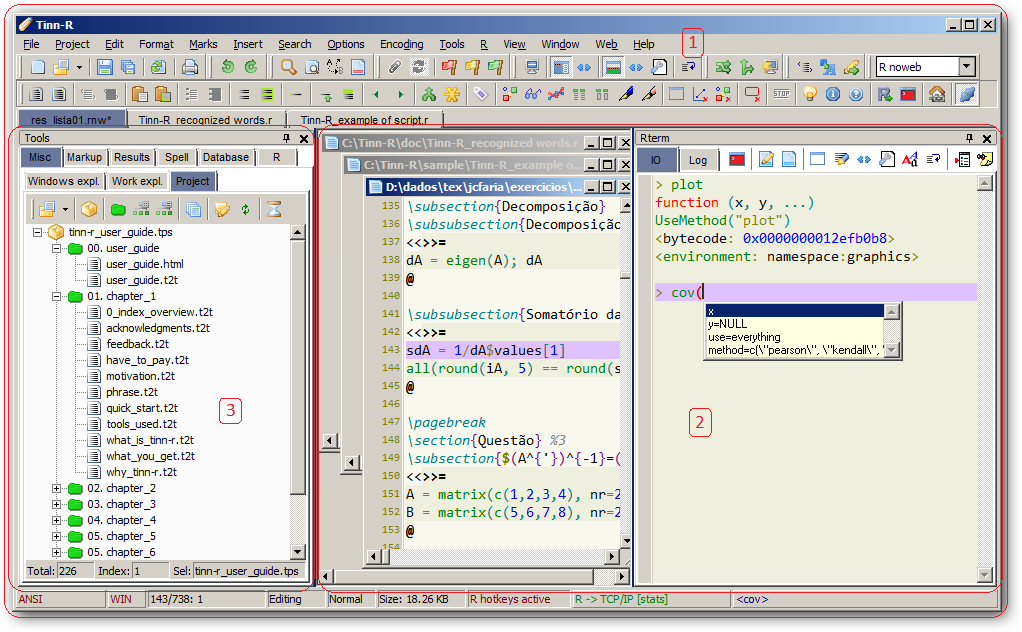
\includegraphics[width=\headwidth]{./res/parts_01.png}
  \end{center}
  \caption{Tinn-R: Main resources.}
  \label{fig:tinn-r_interface}
\end{figure}

Tinn-R interface
(Figure \ref{fig:tinn-r_interface})
is very flexible and user configurable. It is necessary time
to know all available resources and to configure this out (according to your
preferences) in a nice way. The default set of options might not be suitable
for every user.

The window \textit{Application options} allows the user to set the major piece
of user preferences related to the application.

It must be clear from now on that the Tinn-R project is the sum of three main
resources (Figure \ref{fig:tinn-r_interface}):
The application \texttt{per se (1)},
the instances of the \texttt{SynEdit class (2)}
and additional \texttt{Tools (3)},
the latest one projected to allows the expansion of resources.
\index{application options}

The options visible in all pictures reflect a set of the project coordinator
preferences.


\hypertarget{working_app_main}{}
\subsection{Main}
\index{application options!main}

\begin{figure}[h!]
  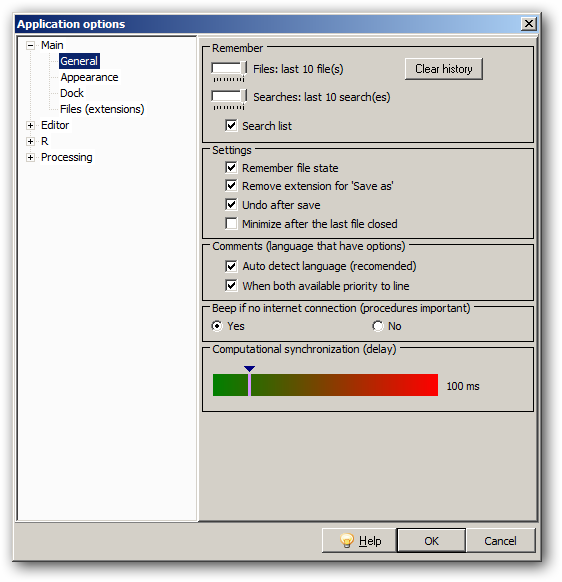
\includegraphics[scale=0.35]{./res/app_main_general.png}~~
  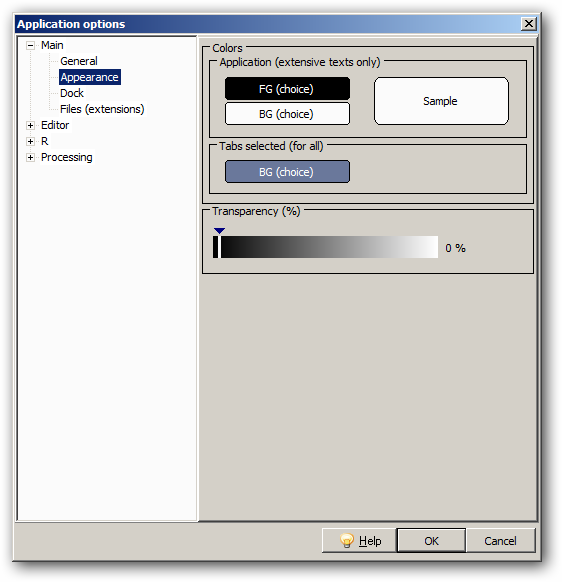
\includegraphics[scale=0.35]{./res/app_main_appearance.png}\\
  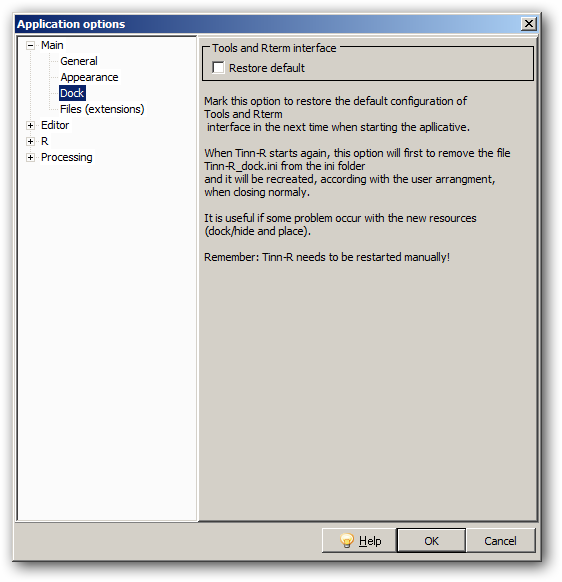
\includegraphics[scale=0.35]{./res/app_main_dock.png}~~
  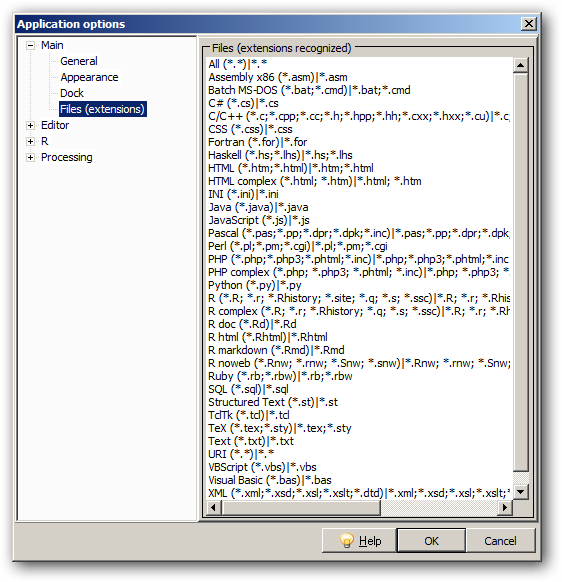
\includegraphics[scale=0.35]{./res/app_main_files.png}\\
  \caption{Main (Options/Application).}
  \label{fig:app_main_options}
\end{figure}

\begin{table}
  \begin{footnotesize}
    \begin{tabularx}{\headwidth}{>{\hsize=0.35\hsize}X>{\hsize=0.65\hsize}X}\\
      \hline
      \textbf{Option} & \textbf{Description} \\
      \hline
      Computational syncronization (delay) & Several processes are dependent on synchronization between applications
       (\RR{}, converters, compilers). The optimal value of the delay is determined by the following characteristics:
       user habits, hardware and software available.
       The ideal value is unique to the various possible combinations of those three characteristics.
       Try to reduce to the minimum value (50 ms) and test it: if something does not work, increase it gradually
       and keep testing until getting to the optimal value. The default value (100 ms) may not be optimal for all users. \\
      Remove extension for \textit{Save as} & All file extensions will be removed
       in the \textit{Save as} Windows interface \\
      Application colors (extensive text only) & Dark colors (low level of radiation)
       for the background, and pale light (high level of radiation) for the characters
       are reccomended for people who work with the computer/monitor for long periods.
       Pictures of this user guide ire like this \\
      \hline
    \end{tabularx}
  \end{footnotesize}
  \caption{Same main options}
  \label{tab:app_main}
\end{table}

Figure \ref{fig:app_main_options} and
Table \ref{tab:app_main}
show the options related to this topic.

Since the options are self-explanatory, Table \ref{tab:app_main} only gives some
details about the most difficult options to understand.


\hypertarget{working_app_r}{}
\subsection{R}
\index{application options!R}

\begin{figure}[h!]
  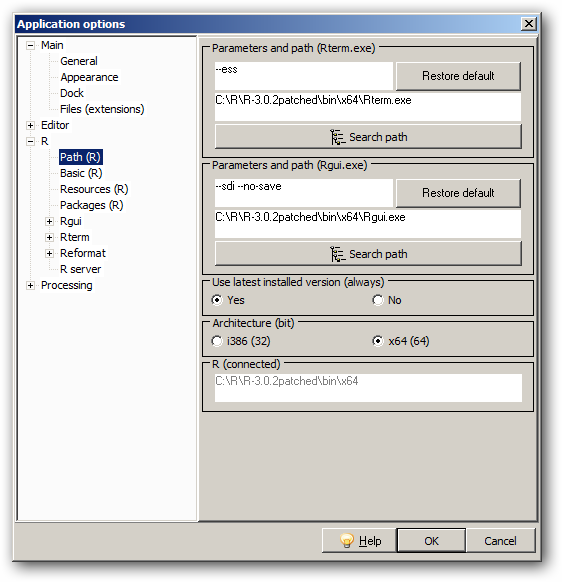
\includegraphics[scale=0.35]{./res/app_r_path.png}~~
  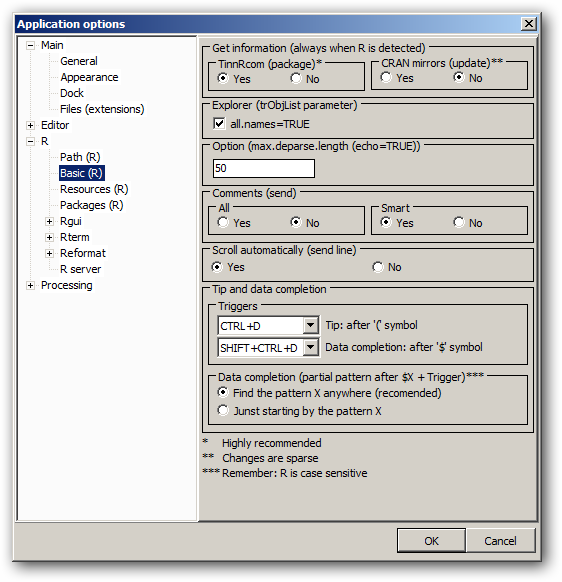
\includegraphics[scale=0.35]{./res/app_r_basic.png}\\
  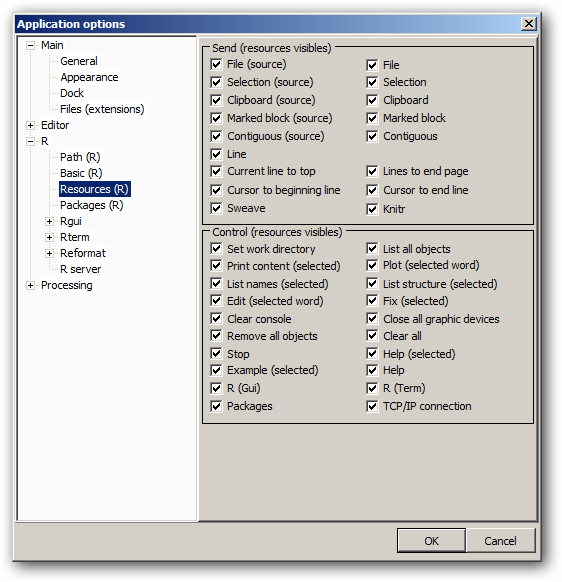
\includegraphics[scale=0.35]{./res/app_r_resources.png}~~
  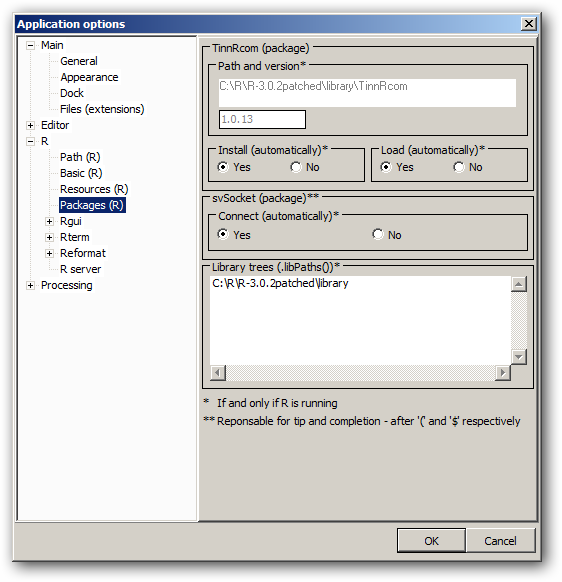
\includegraphics[scale=0.35]{./res/app_r_packages.png}\\
  \caption{R (Options/Application).}
  \label{fig:app_r_a}
\end{figure}

\begin{figure}[h!]
  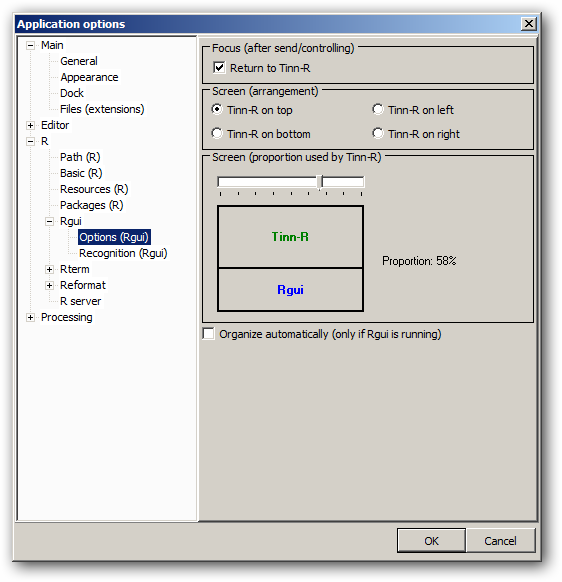
\includegraphics[scale=0.35]{./res/app_r_rgui_options.png}~~
  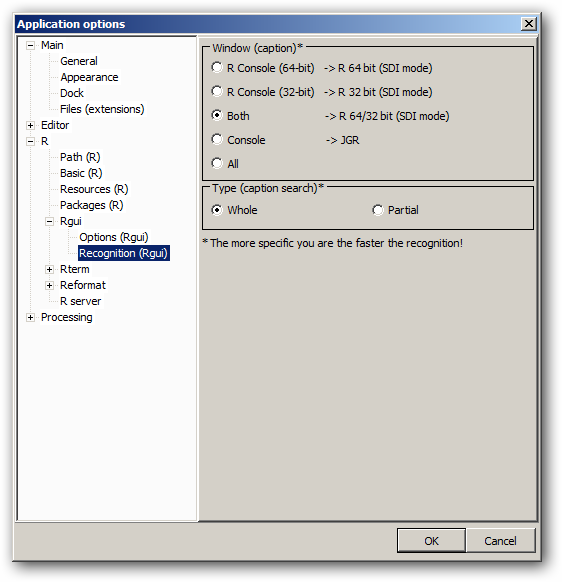
\includegraphics[scale=0.35]{./res/app_r_rgui_recognition.png}\\
  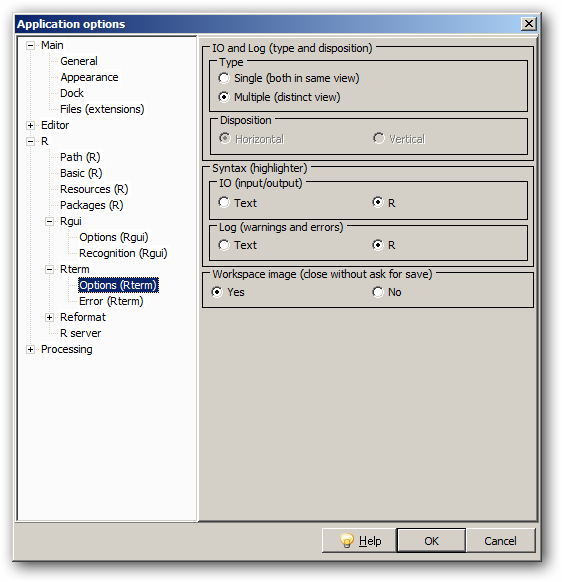
\includegraphics[scale=0.35]{./res/app_r_rterm_options.png}~~
  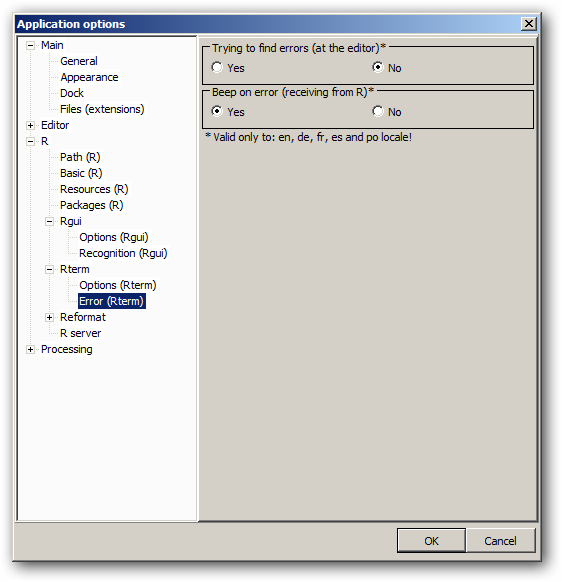
\includegraphics[scale=0.35]{./res/app_r_rterm_error.png}\\
  \caption{R (Options/Application).}
  \label{fig:app_r_b}
\end{figure}

\begin{figure}[h!]
  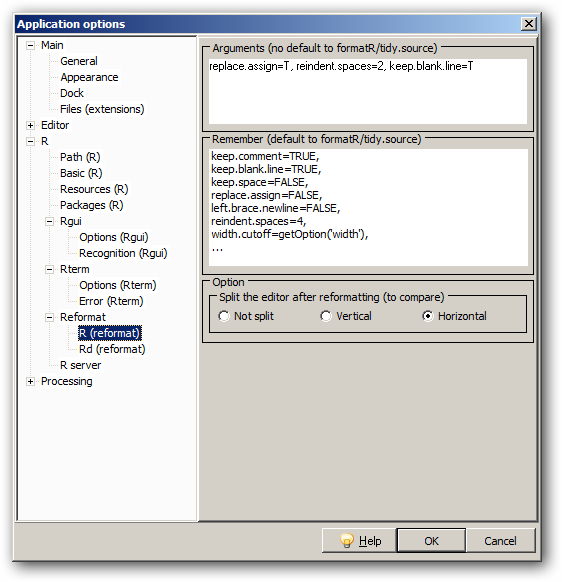
\includegraphics[scale=0.33]{./res/app_r_reformat_r.png}~~
  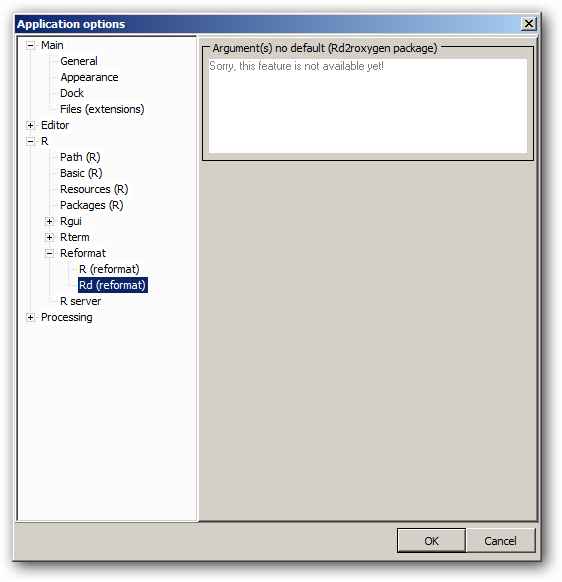
\includegraphics[scale=0.33]{./res/app_r_reformat_rd.png}~~
  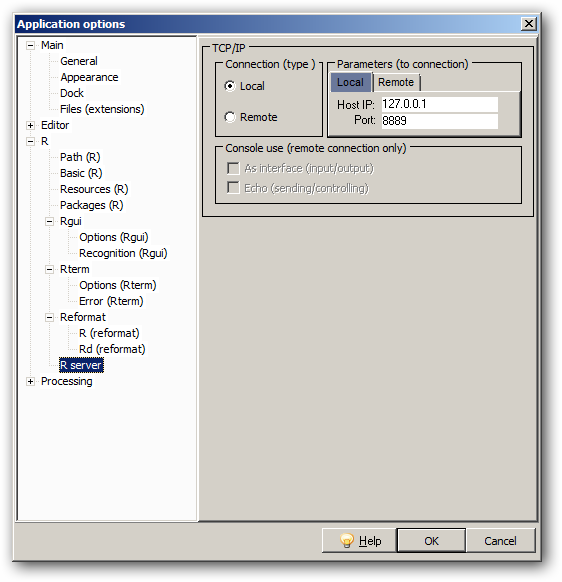
\includegraphics[scale=0.33]{./res/app_r_server.png}\\
  \caption{R (Options/Application).}
  \label{fig:app_r_c}
\end{figure}

Figures \ref{fig:app_r_a}, \ref{fig:app_r_b} and \ref{fig:app_r_c}
shows a set of options available. As you can see, it allows a high level
of customization with the \RR{} environment.


\hypertarget{working_app_processing}{}
\subsection{Processing}
\index{application options!processing}

\begin{figure}[h!]
  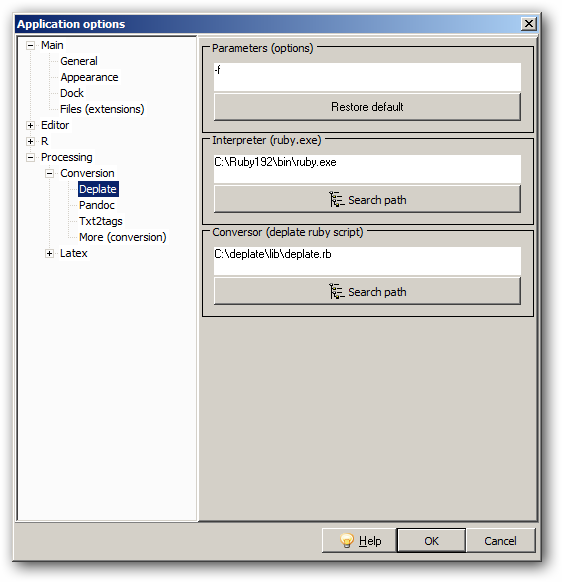
\includegraphics[scale=0.35]{./res/app_processing_conversion_deplate.png}~~
  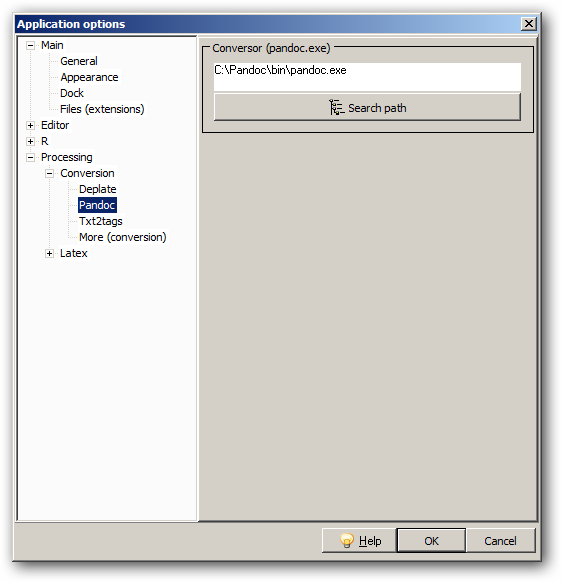
\includegraphics[scale=0.35]{./res/app_processing_conversion_pandoc.png}\\
  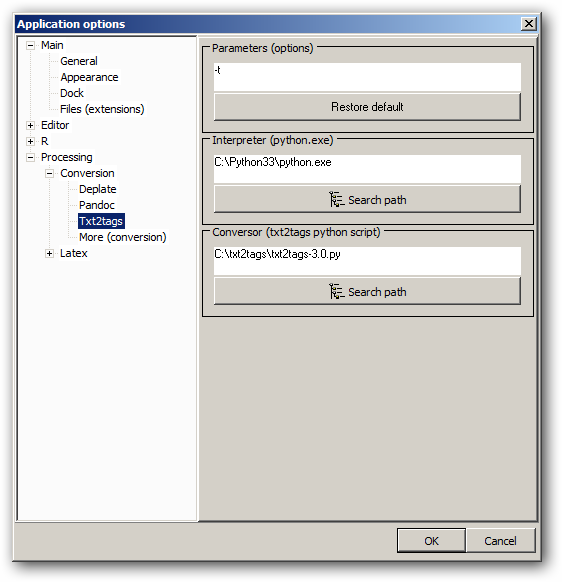
\includegraphics[scale=0.35]{./res/app_processing_conversion_txt2tags.png}~~
  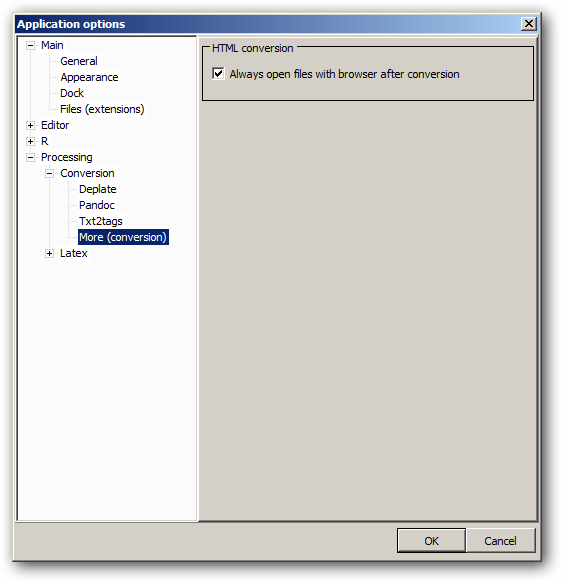
\includegraphics[scale=0.35]{./res/app_processing_conversion_more.png}\\
  \caption{Conversion (Options/Application/Processing).}
  \label{fig:app_processing_conversion_options}
\end{figure}

There are resources
(Figure \ref{fig:app_processing_conversion_options} and
\ref{fig:app_processing_latex_options})
related to conversion (Deplate, Pandoc and Txt2tags) and compilation (Miktex).


\hypertarget{working_app_processing_conversion}{}
\subsubsection{Conversion:}
\index{application options!processing conversion}

Tinn-R project makes it easy to work with these nice conversion tools: Deplate, Pandoc and Txt2tags.
(Figure \ref{fig:app_processing_conversion_options}).


\newpage
\hypertarget{working_app_processing_latex}{}
\subsubsection{LaTex:}
\index{application options!processing LaTeX}

\begin{figure}[h!]
  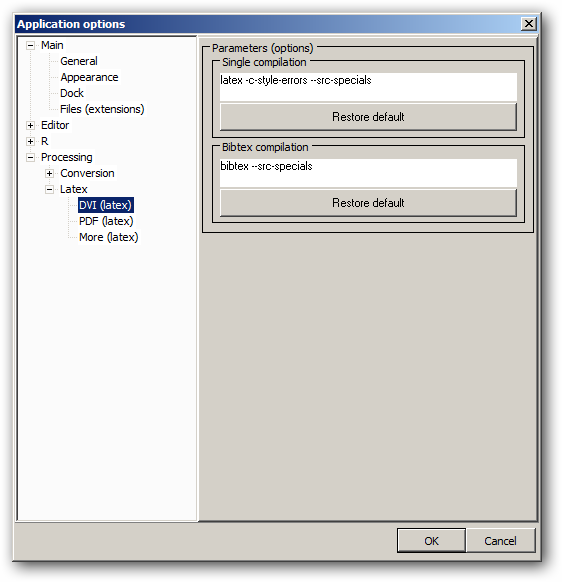
\includegraphics[scale=0.33]{./res/app_processing_latex_dvi.png}~~
  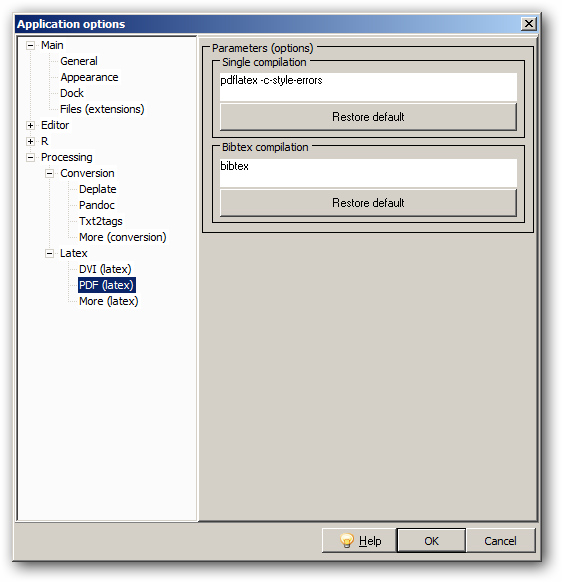
\includegraphics[scale=0.33]{./res/app_processing_latex_pdf.png}~~
  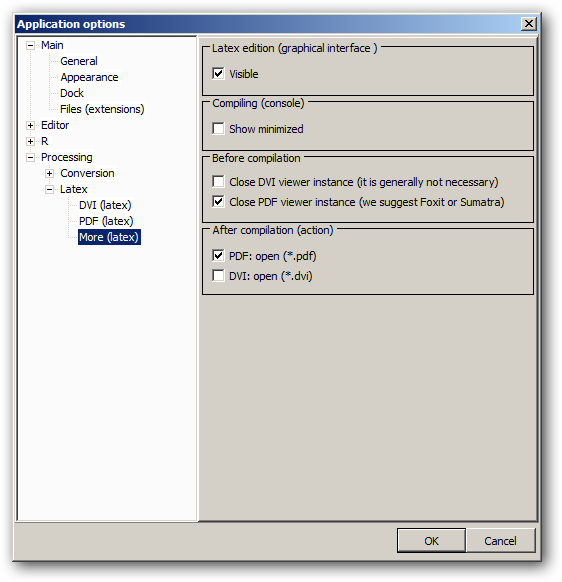
\includegraphics[scale=0.33]{./res/app_processing_latex_more.png}\\
  \caption{Latex (Options/Application/Processing).}
  \label{fig:app_processing_latex_options}
\end{figure}

Tinn-R is not a specific editor to \LaTeX, but it has the basic resources (Figure \ref{fig:app_processing_latex_options}) allowing the user to use the main resources of this environment.

\newpage

\hypertarget{working_editor}{}
\section{Editor options}
\index{editor options}

The \textit{Editor options} window
(Figures \ref{fig:editor_display}, \ref{fig:editor_advanced} and \ref{fig:editor_keystrokes})
was adapted from the sources of the
\textit{SynEdit} component, mainly related to the general appearance and
standard options. The set of options available complement the
\textit{Application options} and allows high level of customization.


\hypertarget{working_editor_display}{}
\subsection{Display}
\index{editor options!display}

\begin{figure}[h!]
  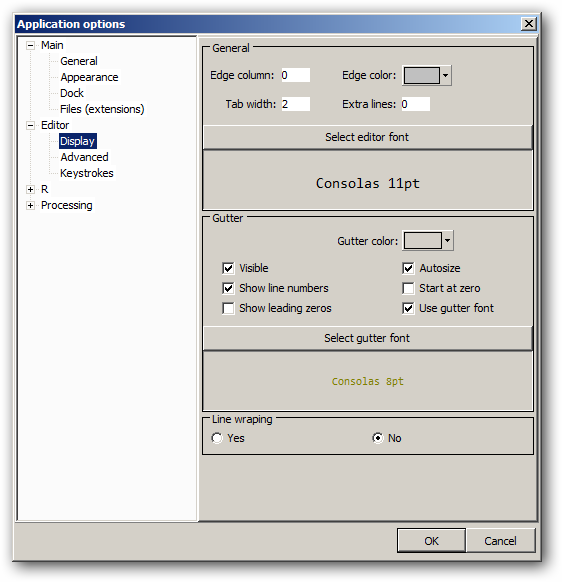
\includegraphics[scale=0.50]{./res/app_editor_display.png}~~
  \caption{Editor options: Display.}
  \label{fig:editor_display}
\end{figure}

\begin{table}
  \begin{footnotesize}
    \begin{tabularx}{\textwidth}{>{\hsize=0.3\hsize}X>{\hsize=0.7\hsize}X}\\
      \hline
      \textbf{Option} & \textbf{Description} \\
      \hline  %Display-----
      Edge column & Will be showed as a vertical line in the editor and the default is 80 characters.
      Set it to 0 or a negative value (-1) to make the edge column not visible \\
      Edge color & Choice of the edge color \\
      Tab width & Set the number of characters that will be inserted when typing the \textit{Tab} key \\
      Extra lines & Set the width which each single line will be displayed \\
      Font & Will open the Windows interface for choosing installed fonts \\
      \hline %Gutter-----
      Gutter color & Will open the Windows interface to choose a color \\
      Visible & Visibility option \\
      Autosize & Autosize option \\
      Show line number & Show line number option \\
      Start at zero & Start at zero option \\
      Show leading zeros & Show leading zeros option \\
      Use gutter font & Use gutter font option \\
      \hline
    \end{tabularx}
  \end{footnotesize}
  \caption{Display (Options/Editor).}
  \label{tab:editor_display}
\end{table}

Figure \ref{fig:editor_display} and
Table \ref{tab:editor_display}
show the main resources.

\hypertarget{working_editor_advanced}{}
\subsection{Advanced options}
\index{editor options!advanced}

\begin{figure}[h!]
  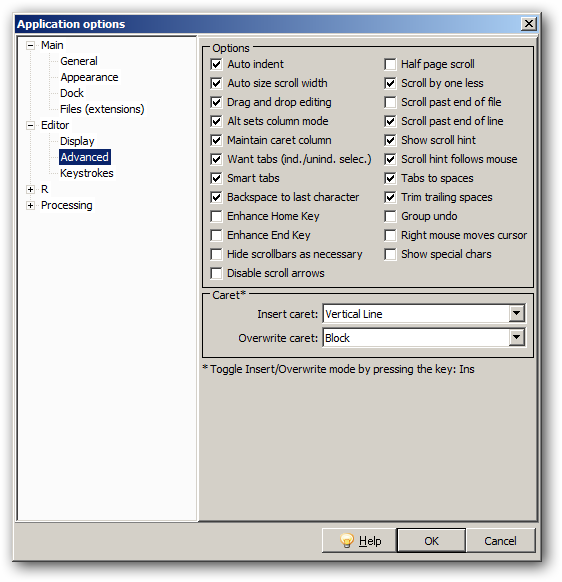
\includegraphics[scale=0.50]{./res/app_editor_advanced.png}~~
  \caption{Editor options: Advanced.}
  \label{fig:editor_advanced}
\end{figure}

\begin{table}
  \begin{footnotesize}
    \begin{tabularx}{\headwidth}{lX}\\
      \hline
      \textbf{Option} & \textbf{Description} \\
      \hline %Options-----
      Auto indent & Will indent the caret (position of the cursor in the current line) on new lines with the same amount of leading white space as the preceding line \\
      Auto size scroll width & Automatically resizes the MaxScrollWidth property when inserting text \\
      Drag and drop editing & Allows you to select a block of text and drag it within the document to another location \\
      Alt sets column mode & Holding down the $<$ALT$>$ key will put the selection mode into column format \\
      Maintain caret column & When moving through lines w/o cursor past EOL, keeps the X position of the cursor \\
      Want tabs & When active $<$TAB$>$ and $<$SHIFT$>$$<$TAB$>$ act as block indent, unindent when text is selected \\
      Smart tabs & When tabbing, the cursor will go to the next non-white space character of the previous line \\
      Smart tab delete & Similar to Smart Tabs, but when you delete characters \\
      Enhance home key & Enhances HOME key positioning, similar to visual studio \\
      Enhance end Key & Enhances END key positioning, similar to JDeveloper \\
      Hide scrollbars as necessary & If enabled, then the scrollbars will only show when necessary.
      If you have ScrollPastEOL, then the horizontal bar will always be there (it uses MaxLength instead) \\
      Disable scroll arrows & Disables the scroll bar arrow buttons when you can't scroll in that direction any more \\
      Half page scroll & When scrolling with page-up and page-down commands, only scroll a half page at a time \\
      Scroll by one less & Forces scrolling to be one less \\
      Scroll past end of file & Allows the cursor to go past the end of file marker \\
      Scroll past end of line & Allows the cursor to go past the last character into the white space at the end of a line \\
      Show scroll hint & Shows a hint of the visible line numbers when scrolling vertically \\
      Scroll hint follows mouse & The scroll hint follows the mouse when scrolling vertically \\
      Tabs to spaces & Converts a tab character to a specified number of space characters \\
      Trim trailing spaces & Spaces at the end of lines will be trimmed and not saved \\
      Group undo & When undoing/redoing actions, handle all continuous changes of the same kind in one call instead undoing/redoing
      each command separately \\
      Right mouse moves cursor & When clicking with the right mouse for a pop-up menu, move the cursor to that location \\
      Show special chars & Shows the special characters \\
      \hline %Caret-----
      Insert caret & A list with four options: Vertical line, Horizontal line, Half block and block \\
      Overwrite caret & A list with options: Vertical line, Horizontal line, Half block and block \\
      \hline
    \end{tabularx}
  \end{footnotesize}
  \caption{Display (Options/Editor).}
  \label{tab:editor_advanced}
\end{table}

Figure \ref{fig:editor_advanced} and
Table \ref{tab:editor_advanced}
show the main resources.


\hypertarget{working_editor_keystrokes}{}
\subsection{Keystrokes}
\index{editor options!keystrokes}

\begin{figure}[h!]
  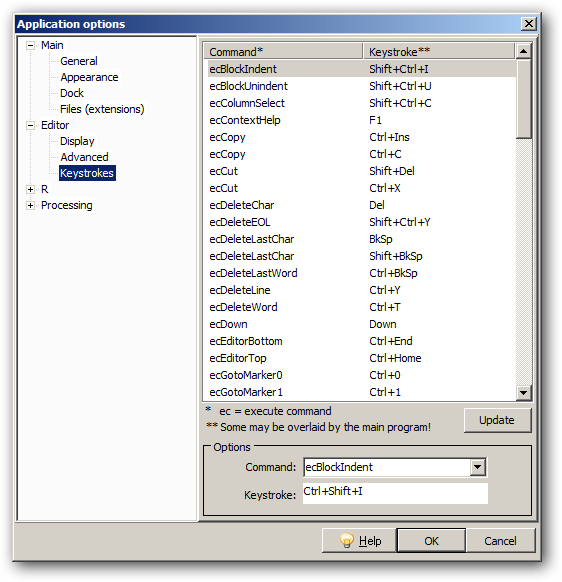
\includegraphics[scale=0.50]{./res/app_editor_keystrokes.png}\\
  \caption{Editor options: keystrokes.}
  \label{fig:editor_keystrokes}
\end{figure}

This interface
(Figure \ref{fig:editor_keystrokes})
allows to change the default SynEdit keystrokes.
It is possible to make new, edit or remove any ecAction (execute command action).
A set of user friendly keystrokes gives high productivity leading with
all instances of the main class \textit{SynEdit}: Editor, IO and Log.

\newpage

\hypertarget{working_selectionmode}{}
\section{Selection mode}
\index{selection mode}

Allows the setting of the current selection mode
(Figure \ref{fig:selection_normal},
\ref{fig:selection_line} and
\ref{fig:selection_column}).

Select text by clicking and dragging with the left mouse button held
down or moving the cursor with the shift key held down. The status
bar will display an icon indicating the current selection mode.

\hypertarget{working_selectionmode_normal}{}
\subsection{Normal}
\index{selection mode!normal}

\begin{figure}[h!]
  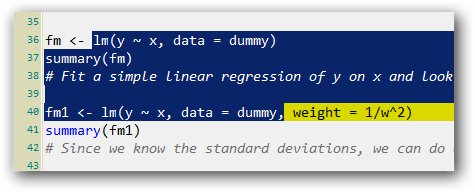
\includegraphics[scale=0.35]{./res/selection_normal.png}\\
  \caption{Normal (selection mode).}
  \label{fig:selection_normal}
\end{figure}

This is the standard selection mode
(Figure \ref{fig:selection_normal})
found in many Windows applications.

\hypertarget{working_selectionmode_line}{}
\subsection{Line}
\index{selection mode!line}

\begin{figure}[h!]
  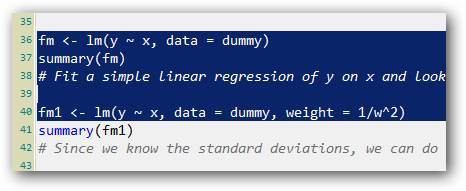
\includegraphics[scale=0.35]{./res/selection_line.png}\\
  \caption{Line (selection mode).}
  \label{fig:selection_line}
\end{figure}

This selection mode
(Figure \ref{fig:selection_line})
allows only for complete lines to be selected.

\hypertarget{working_selectionmode_column}{}
\subsection{Column}
\index{selection mode!column}

\begin{figure}[h!]
  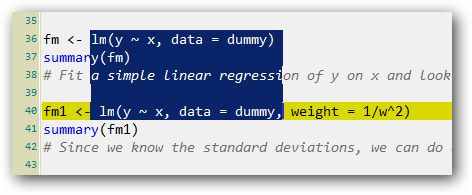
\includegraphics[scale=0.35]{./res/selection_column.png}\\
  \caption{Column (selection mode).}
  \label{fig:selection_column}
\end{figure}

This selection mode
(Figure \ref{fig:selection_column})
allows vertical blocks of text to be selected.
The option \texttt{ALT} sets column mode allowing the selection
mode to be switched to Column Mode when selecting with the mouse
by simply holding down the \texttt{ALT} key.
\htmladdnormallink{See details at editor (advanced options)}{\#working_editor_advanced}.

\newpage

\hypertarget{working_highlighters}{}
\section{Highlighters (settings)}
\index{highlighters!color}

\begin{figure}[h!]
  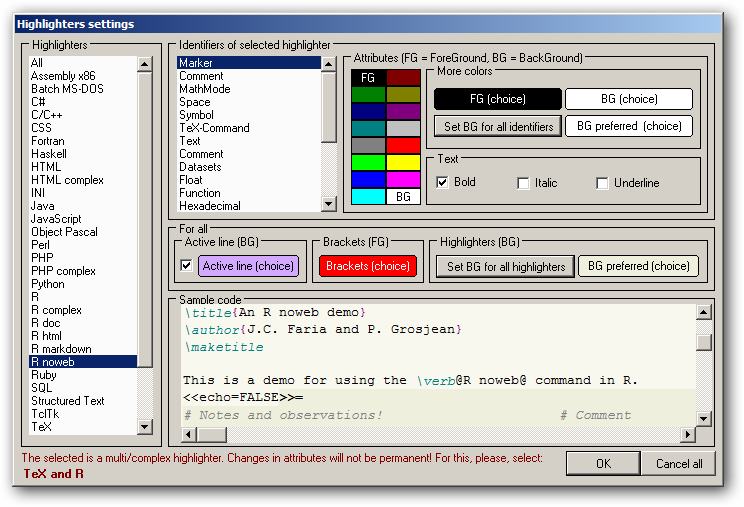
\includegraphics[scale=0.50]{./res/highlighter_settings.png}\\
  \caption{Highlighter preferences.}
  \label{fig:highlighter_preferences}
\end{figure}

This interface
(Figure \ref{fig:highlighter_preferences})
allows you to customize the appearance and colors of the
instances of the class \textit{SynEdit} (Editor, IO and Log).

The interface is simple and self-explanatory.

Basically, make a choice between the set of highlighters available
from the \textit{Highlighters} list. The identifier of the selected
highlighter will be updated. It is possible to set only one
foreground attribute each time. But it is possible to set the
background for all attributes of the selected highlighter and also
the background of all attributes of all highlighters.

It is also possible to set the color brackets and the active line
background.


\subsubsection{Observation:}
\index{highlighters!multi-highlighters}
Tinn-R has seven multi-highlighters: \textit{HTML complex}, \textit{PHP complex},
\textit{R complex}, \textit{R doc},  \textit{R html}, \textit{R markdown} and \textit{R noweb},
with each one behaving as follows:

\begin{footnotesize}
  \begin{verbatim}
    1. HTML complex = HTML & JavaScript
    2. PHP complex  = HTML & JavaScript & PHP
    3. R complex    = R & URI ('<<<' begin URI; '>>>' end URI)
    4. R doc        = TeX & R ('>>=' begin R; '@' end R)
    5. R html       = HTML & R ('<!--begin.rcode' begin R; 'end.rcode-->' end R)
    5. R markdown   = URI & R ('```{' begin R; '```' end R)
    6. R noweb      = TeX & R ('>>=' begin R; '@' end R)

    URI       : Uniform Resource Identifiers.

    R complex : The main syntax is R, '<<<' and '>>>' are the tags enabling
                the user to insert a block of URI syntax.

    R doc     : The main syntax is TeX, '>>=' and '@' are the tags enabling
                the user to insert a block of R syntax.

    R html    : The main syntax is HTML, '<!--begin.rcode' and 'end.rcode-->' are the tags enabling
                the user to insert a block of R syntax.

    R markdown: The main syntax is URI, '```{' and '```' are the tags enabling
                the user to insert a block of R syntax.

    R noweb   : The main syntax is TeX, '>>=' and '@' are the tags enabling
                the user to insert a block of R syntax.

  \end{verbatim}
\end{footnotesize}

These highlighters haven't priorities when you set the syntax color preferences.
Thus, if you change the colors' preferences of any of these multi-highlighters
these settings will be valid only in the current Tinn-R session and will not be
saved when Tinn-R is closed. So, if you want to make permanent changes, set the
preferences from all simple highlighters.

From version 3.0.1.0 a warning message is displayed whenever
a multi-highlighter is selected. It shows which highlighters the user
must change the characteristics so that they are properly stored and
henceforth always displayed.

\newpage

\hypertarget{working_shortcuts}{}
\section{Shortcuts customization}
\index{shortcuts}
\index{shortcuts!customization}

\begin{figure}[h!]
  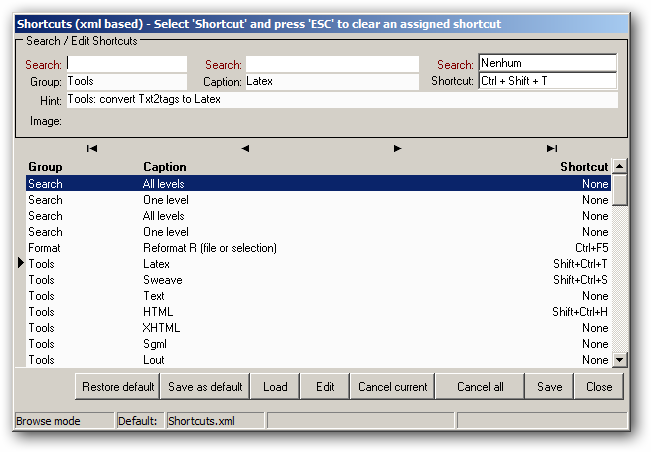
\includegraphics[scale=0.35]{./res/shortcuts_dlg.png}\\
  \caption{Shortcuts customization.}
  \label{fig:shortcuts_dlg_1}
\end{figure}

The \textit{Shortcuts customization}
(Figure \ref{fig:shortcuts_dlg_1})
allows the user to set the shortcuts related
to the application, it works together with the \textit{Editor keystrokes},
and allows for high level of customization.

The difference between \textit{Shortcuts} and \textit{Hotkeys (operational system)}
is that the former works only with the focus on Tinn-R, whereas hotkeys work
with the focus anywhere.

Read below a brief description of available buttons.

\begin{quote}
  \begin{footnotesize}
    \begin{description}
      \item[Restore default:]
        Restores the file \texttt{Shortcuts.xml} from the origin
        (InstallPath/data/data.zip). Any prior changes to the file
        \texttt{Shortcuts.xml} in use will be lost.
      \item[Save as default:]
        Opens the save dialog allowing to save the file. From this
        point, this file will be the new default shortcuts.
      \item[Load:]
        Opens the open dialog allowing to load a shortcut file. From this
        point on, this file will be the new default shortcuts.
      \item[Edit:]
        Sets the table in edition mode.
      \item[Cancel current:]
        Cancels any changes made to the current edition.
      \item[Cancel all:]
        Cancels all changes made to the database prior to \textit{Save}
        or \textit{Save as default}.
      \item[Save:]
        Saves to text file (XML) all changes made to the current table.
      \item[Close:]
        Closes the dialog. All changes not saved will be lost.
    \end{description}
  \end{footnotesize}
\end{quote}

\newpage

\hypertarget{working_hotkeys}{}
\section{Hotkeys (operational system)}
\index{hotkeys}

\begin{figure}[h!]
  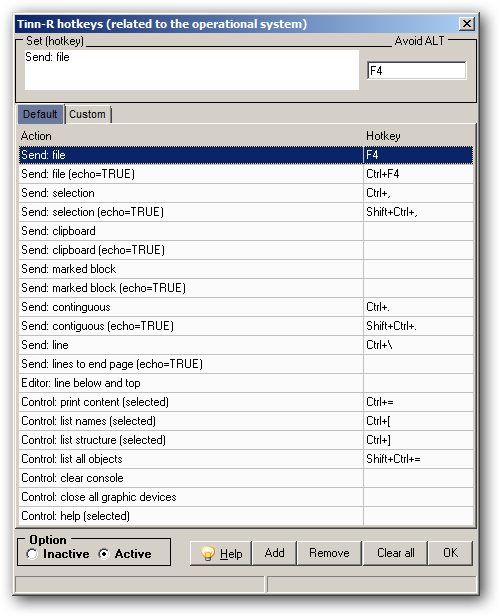
\includegraphics[scale=0.35]{./res/hotkeys_default.png}~~
  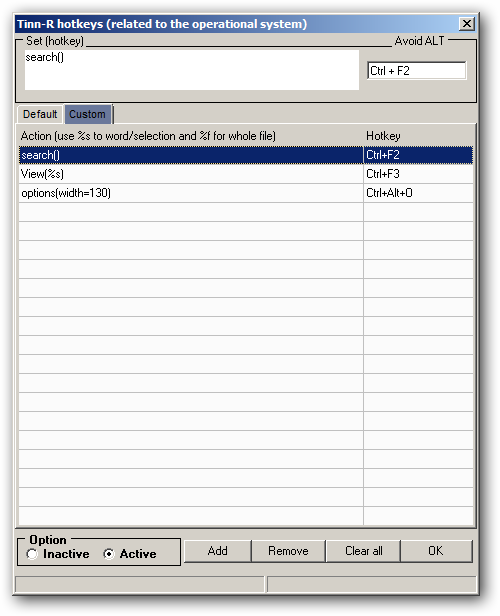
\includegraphics[scale=0.35]{./res/hotkeys_custom.png}
  \caption{Hotkeys.}
  \label{fig:hotkeys}
\end{figure}

The \textit{Hotkeys (operational system)}
(Figure \ref{fig:hotkeys})
allow setting the hotkeys
related to the operational system. The difference between those hotkeys and
\textit{Shortcuts customization} is that the latter works only with the
focus in Tinn-R, whereas the hotkeys work with the focus anywhere.

The interface is self-explanatory. Basically you first make a choice from
the \textit{R/Hotkeys (operational system)} and set the desired Hotkey.

The set of hotkeys will perform actions only if the option \textit{Active}
is checked. The objective of these options (\textit{Inactive} and
\textit{Active}) is to avoid conflict with others applications allowing
to enable/disable the set of hotkeys quickly and easily.

The \texttt{R/Hotkeys} interface was deeply reworked in the version 2.4.0.0 and it now has two tabs,
\texttt{Default} and \texttt{Custom}:

\begin{itemize}
\item \texttt{Default}: Contains the already traditional instructions of Tinn-R;
\item \texttt{Custom}: \textbf{Allows the user to customize any instructions} to be send to \RR{} interpreter (thanks to Philemon Lenherr for the suggestion). The instructions must be as follows:
 \begin{itemize}
 \item Simple: \texttt{search()}. The \RR{} interpreter will receive \texttt{$>$ search()};
 \item Replace word or small selection: \texttt{View(\%s, title='View of iris dataset')}.
   If the editor cursor is over the word \texttt{iris} or it is selected,
   the \RR{} interpreter will receive \texttt{$>$ View(iris, title='View of iris dataset')}
 \item Replace whole file: \texttt{source(\%f, echo=TRUE, verbose=TRUE)}.
   The \RR{} interpreter will receive \texttt{$>$ source(.trPaths[4], echo=TRUE, verbose=TRUE)}.
   All rules related to send file are preserved.
 \end{itemize}
\end{itemize}

\newpage

\hypertarget{working_rterm}{}
\section{Rterm interface}
\index{Rterm!interface}

\begin{figure}[h!]
  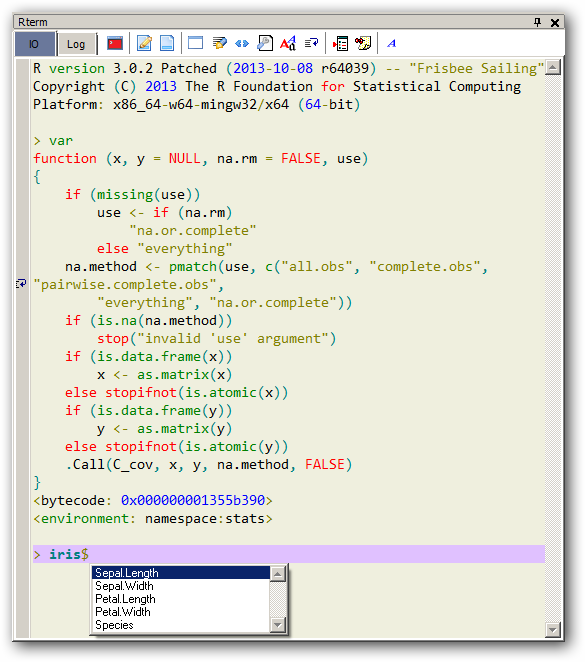
\includegraphics[scale=0.35]{./res/rterm.png}\\
  \caption{Rterm interface.}
  \label{fig:rterm_interface}
\end{figure}

The implementation of a Rterm interface
(Figure \ref{fig:rterm_interface},
\ref{fig:rterm_io} and
\ref{fig:rterm_log})
in Tinn-R has the following aims:
\begin{itemize}
  \item To address some limitations (edition, navigation and control) imposed by the Rgui.exe interface;
  \item To add more flexibility and power to the GUI/Editor;
  \item To maintain the prior user knowledge associated with Tinn-R editor and the Rgui console;
  \item To maintain the structural simplicity of the application;
  \item To use a more efficient engine of Inter Process Communication (IPC)
    than the Windows clipboard used in previous versions.
\end{itemize}

The \textit{IO}
(Figure \ref{fig:rterm_io})
and \textit{Log}
(Figure \ref{fig:rterm_log})
interfaces are instances of the class
SynEdit. In other words, all prior user knowledge of the resources associated with the editor were preserved:
\index{SynEdit}

\begin{itemize}
  \item Free navigation with keyboard keys;
  \item Marks;
  \item Shortcuts;
  \item Syntax;
  \item Match brackets;
  \item Tips;
  \item Data completion;
  \item Edition: copy, paste, cut, etc;
  \item Selection/copy/paste in column mode:
    \texttt{ALT + drag the mouse}, if this option is checked
    (\htmladdnormallink{see editor options}{\#working\_editor}), etc.
\end{itemize}

\begin{enumerate}
  \item \textit{IO} (Figure \ref{fig:rterm_io}): The aim was to add flexibility and power, i.e.,
    joining the power of SynEdit (editor) and the functionality of
    a common console.
  \item \textit{Log} (Figure \ref{fig:rterm_log}): Has three basic objectives:
    \begin{enumerate}
      \item To receive and show warnings and error messages;
      \item To make the \textit{IO} interface cleaner;
      \item To avoid synchronization difficulties with the inter
        process communication (IPC) called \textit{pipe} used.
    \end{enumerate}
\end{enumerate}

When more than one recognized instance of \RR{} is running the priority
order is:

\begin{enumerate}
  \item Rterm;
  \item Rgui;
  \item Rserver (remote);
\end{enumerate}


\hypertarget{working_rterm_io}{}
\subsection{IO}
\index{IO Interface}

\begin{figure}[h!]
  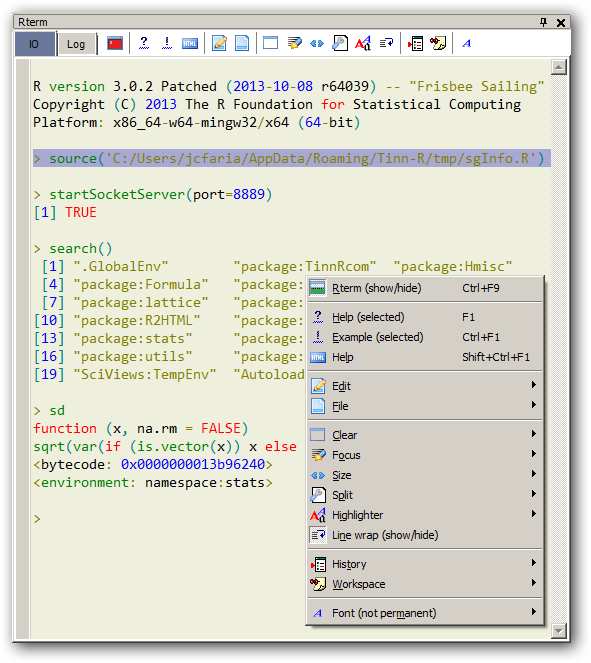
\includegraphics[scale=0.35]{./res/rterm_io.png}\\
  \caption{IO (Rterm interface).}
  \label{fig:rterm_io}
\end{figure}

\begin{table}
  \begin{footnotesize}
    \begin{tabularx}{\textwidth}{>{\hsize=0.3\hsize}X>{\hsize=0.7\hsize}X}\\
      \hline
      \textbf{Resource} & \textbf{Description} \\
      \hline
      Edition & All resources available to the editor (copy, paste, cut, etc) can be used \\
      Free navigation & Using keyboard keys: Home, Page Up, Page Down, End, Left, Top, Right and Bottom \\
      Marks & \texttt{CTRL + [0..9]} can be used to mark, \texttt{SHIFT + CTRL + [0..9]} to go to prior marks \\
      Shortcuts & All shortcuts available to the editor are also to the IO \\
      Syntax & Two options: Text and \RR{} \\
      Match brackets & Makes it easier to build more complex instructions like \texttt{plot(sqrt(rnorm(1e3)), pch='.', cex=3)} \\
      Tips & Are invoked using the same trigger as the editor \\
      Data completion & Are invoked using the same trigger as the editor \\
      \hline
      \\
    \end{tabularx}
  \end{footnotesize}
  \caption{IO interface, main resources available.}
  \label{tab:io_interface}
\end{table}

The \textit{IO} interface
(Figure \ref{fig:rterm_io} and
Table \ref{tab:io_interface})
is used to receive output (SDTOUT) from the \RR{} environment.

It is necessary to adjust some \RR{} options (for example: \texttt{options(width=70)}
to obtain a suitable number of characters in each single line, according to
hardware and user preferences (side of \textit{IO}, place of \textit{IO},
length of \textit{IO}, width of \textit{IO}, type and size of font). Once
you get a suitable result, it is a good practice to add this option to the
\texttt{Rprofile.site} (located inside of the folder \textit{etc} where the
\RR{} was installed) file. Thus, your option will always be set when
starting \RR{}.

The IO is an instance of SynEdit. Therefore, it can be edited and used like
the editor, allowing the tasks showed in the
Table \ref{tab:io_interface}.

If the \textit{IO} has the focus, all actions of the \RR{} toolbar and main menu
associated with control \RR{} can be used in the IO interface.

The \textit{IO} interface has a special pop-up menu allowing the most common
tasks. It is self-explanatory. So, make a small tour (right mouse button inside
of Rterm/IO) to find out about its options.

Some details:

\begin{itemize}
  \item Shortcuts and pop-up menu make it easy to change among the interfaces:
    \textit{Editor}, \textit{IO} and \textit{Log}:
    \begin{enumerate}
      \item if \textit{IO} and \textit{Log} are in distinct tabs (views), the
        common Windows shortcut \texttt{CTRL + TAB} changes the active page (IO-Log).
      \item Any prior line can be sent another time by just putting the cursor
        in any place of it and typing: \texttt{CTRL + ENTER};
    \end{enumerate}
  \item The last line of the \textit{IO} interface (the prompt) has special features:
    \begin{enumerate}
      \item It has some restrictions for edition and navigation;
      \item \texttt{ALT+DOWN} and \texttt{ALT+UP} are the shortcuts (prior/later)
        for command history. The history is continuous, cyclic, and have a 100
        line limit.
    \end{enumerate}
\end{itemize}


\hypertarget{working_rterm_log}{}
\subsection{Log}
\index{Rterm!Log}

 \begin{figure}[h!]
  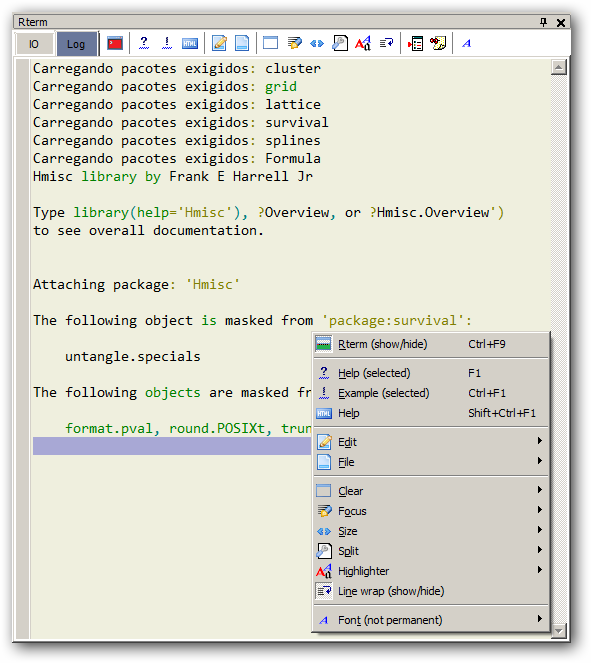
\includegraphics[scale=0.35]{./res/rterm_log.png}\\
  \caption{Log (Rterm interface).}
  \label{fig:rterm_log}
\end{figure}

The \textit{Log} interface
(Figure \ref{fig:rterm_log})
is used to receive warnings and error messages (SDTERR) from the \RR{} environment.

It has a special pop-up menu that allows the most common tasks. It is
self-explanatory. So, take a small tour (right mouse buttom inside of
Rterm/Log) to know all options.

Most of the resources available to the \textit{IO} are also available to this
interface.

\newpage

\hypertarget{working_tools}{}
\section{Tools interface}
\index{tools}
\index{tools!interface}

This graphical interface
(Figure \ref{fig:tools_misc_options})
was projected to allow access to Tinn-R resources
and also to accommodate future growth of related news resources.

Position: starting from version 2.1.1.1 (Oct/15/2008) this interface is
dockable. It can float or be docked on the left, top, right, or bottom
sides of the main interface.


\hypertarget{working_tools_misc}{}
\subsection{Misc}
\index{tools!misc}

\begin{figure}[h!]
  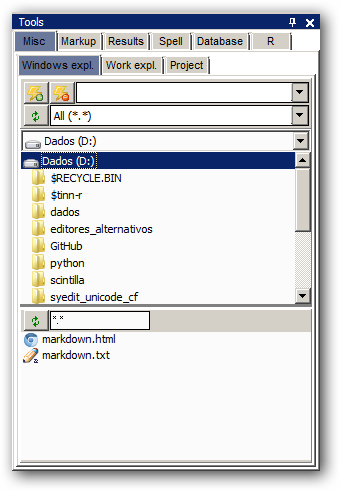
\includegraphics[scale=0.35]{./res/tools_misc_windowsexpl.png}~~
  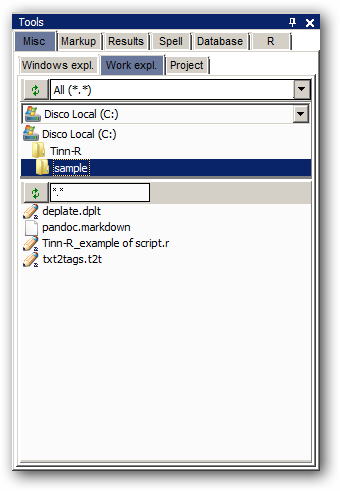
\includegraphics[scale=0.35]{./res/tools_misc_workexpl.png}~~
  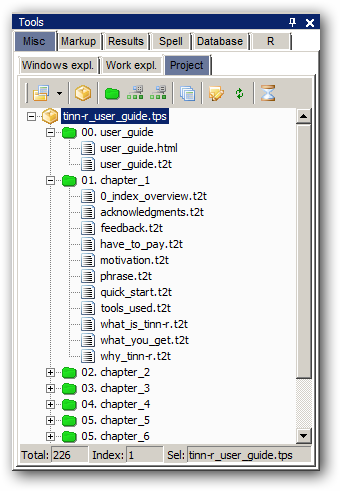
\includegraphics[scale=0.35]{./res/tools_misc_project.png}\\
  \caption{Tools interface.}
  \label{fig:tools_misc_options}
\end{figure}

\begin{table}[h!]
  \begin{footnotesize}
    \begin{tabularx}{\textwidth}{>{\hsize=0.3\hsize}X>{\hsize=0.7\hsize}X}\\
      \hline
      \textbf{Tool} & \textbf{Description} \\
      \hline
      Windows expl. & \textit{\htmladdnormallink{See details ...}{\#working\_tools\_misc\_windowsexpl}} \\
      Work expl. & \textit{\htmladdnormallink{See details ...}{\#working\_tools\_misc\_workexpl}} \\
      Project & \textit{\htmladdnormallink{See details ...}{\#working\_tools\_misc\_project}} \\
      \hline
    \end{tabularx}
  \end{footnotesize}
  \caption{Misc (tools)}
  \label{tab:tools_misc}
\end{table}

The resources are showed in
Figure \ref{fig:tools_misc_options} and
Table \ref{tab:tools_misc}.


\hypertarget{working_tools_misc_windowsexpl}{}
\subsubsection{Windows expl.:}

See Figure \ref{fig:tools_misc_options}.

\begin{itemize}
  \item Allows manager favorites (add and remove);
  \item Allows filter by file extension;
  \item Has pop-up menus similar to Windows explorer;
  \item Support drag and drop actions (it is possible to drag
    any file and drop it on the editor interface to be opened).
\end{itemize}


\hypertarget{working_tools_misc_workexpl}{}
\subsubsection{Work expl.:}

See Figure \ref{fig:tools_misc_options}.

\begin{itemize}
  \item Always shows the folder related to the latest file opened;
  \item Does not have a pop-up menu;
  \item Supports drag and drop actions, i.e, it is possible to drag any
    file and drop it in the editor interface that will be opened.
\end{itemize}


\hypertarget{working_tools_misc_project}{}
\subsubsection{Project:}

See Figure \ref{fig:tools_misc_options}.

\begin{itemize}
  \item Allows for project management using a graphical interface;
  \item Supports drag and drop actions, ie, it is possible to drag
    the entire project, groups, or any file and then drop them
    into the editor interface that will be opened:
    \begin{itemize}
      \item Project: will open all files related to the current project;
      \item Group: will open all files for the selected group;
      \item File: will open the selected file.
    \end{itemize}
  \item It is possible to send an entire project,
    a selected group, or an individual file to the \RR{} environment through a pop-up menu.
  \item  Source file of project:
    \begin{itemize}
      \item It is possible to edit the project in text mode (with the button
        \textit{Project: edit (as text file)} of the specific toolbar).
        After any change, save the text file (it contains the textual
        description of the project structure) and reload the file to the
        graphical interface (with the button \textit{Project:
          reload (from text file)} of the specific toolbar).
      \item Any changes to the graphical interface will be reflected in the
        text file for the project, after it is saved.
      \item The best way to work with projectis (graphics of textual mode)
        depends on the complexity of the actions and the user preference.
        For single tasks, we suggest that you use the graphical mode.
        For complex actions, it is faster to use the textual mode with
        all editor resources.
    \end{itemize}
\end{itemize}


\hypertarget{working_tools_markup}{}
\subsection{Markup}
\index{tools!markup}
\index{tools!markup txt2tags}
\index{tools!markup \LaTeX}

\begin{figure}[h!]
  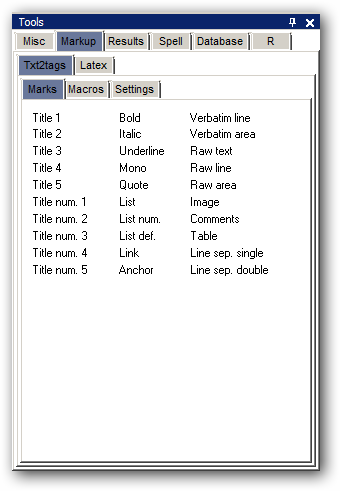
\includegraphics[scale=0.35]{./res/tools_markup_txt2tags_marks.png}~~
  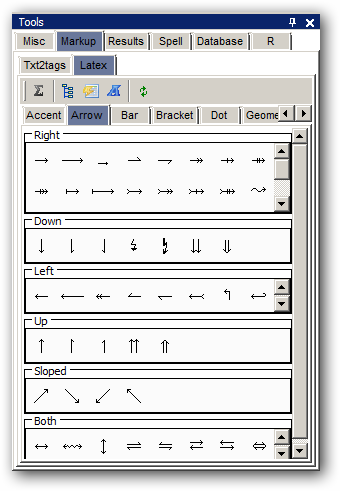
\includegraphics[scale=0.35]{./res/tools_markup_latex_arrows.png}\\
  \caption{Markups (Tools).}
  \label{fig:tools_markup_txt2tags_options}
\end{figure}

\begin{table}
  \begin{footnotesize}
    \begin{tabularx}{\textwidth}{lX}\\
      \hline
      \textbf{Tool} & \textbf{Description} \\
      \hline
      Txt2tags & Sets marks, macros and settings of Txt2tags convertor \\
      Latex & Sets \LaTeX~symbols settings in a customizable manner \\
      \hline
      \\
    \end{tabularx}
  \end{footnotesize}
  \caption{Markup (Tools).}
  \label{tab:tools_markup}
\end{table}

It contains resources
(Figure \ref{fig:tools_markup_txt2tags_options} and
Table \ref{tab:tools_markup})
related to the Txt2tags and \LaTeX.


\subsubsection{Txt2tags:}

Sets
(Figure \ref{fig:tools_markup_txt2tags_options})
marks, macros, and settings for the Txt2tags convertor.
A single click over any graphical will add it to the current editor.


\subsubsection{LaTeX:}

Set
(Figure \ref{fig:tools_markup_txt2tags_options})
of \LaTeX~symbols. A single click over any graphical object
will add it to the current editor;

The symbols, place and order of all symbols are customizable.
To customize them, open the folder \textit{latex} and edit
\textit{ini} path. At the end of the edition, update the interface
using the button \textit{Latex: reload symbols (from ini)}. Be careful
when editing the symbols to maintain the name structure.
For example: \texttt{Number\_SymbolName.FileExtension},
\texttt{001\_alpha.gif}, \texttt{002\_beta.gif}. The number
will be used to order symbols in the graphical interface,
while the name will be used (if recognized) as a \LaTeX~symbol.


\hypertarget{working_tools_results}{}
\subsection{Results}
\index{tools!results}

\begin{table}
  \begin{footnotesize}
    \begin{tabularx}{\textwidth}{>{\hsize=0.3\hsize}X>{\hsize=0.7\hsize}X}\\
      \hline
      \textbf{Tool} & \textbf{Description} \\
      \hline
      Ini log & Displays useful results when starting Tinn-R \\
      Search & Interface for \textit{Search} results associated with \textit{Search in files} \\
      \hline
      \\
    \end{tabularx}
  \end{footnotesize}
  \caption{Results (Tools).}
  \label{tab:tools_results}
\end{table}

It contains resources
(Table \ref{tab:tools_results})
related to \textit{Ini log} and \textit{Search}.


\subsubsection{Ini log:}
\index{tools!results inilog}\\

\begin{figure}[h!]
  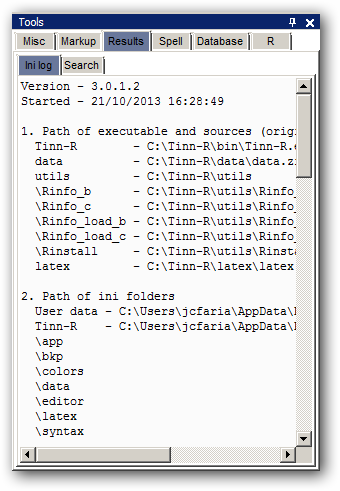
\includegraphics[scale=0.35]{./res/tools_results_inilog.png}\\
  \caption{Inilog (Tools/Results).}
  \label{fig:tools_results_inilog}
\end{figure}

\begin{table}
  \begin{footnotesize}
    \begin{tabularx}{\textwidth}{XX}\\
      \hline
      \textbf{Topic} & \textbf{Description} \\
      \hline
      Path of executable and sources (origin) & Lists executable files and resources \\
      Path of ini files & Lists the path of all folders of the ini \\
      Verification of necessary folder and files & Lists the status of folders and files of ini \\
      Tinn-R, bkp, colors, ini, syntax and syntax bkp & Lists the status of these folders \\
      Custom (version) & Lists the status of this folder and files \\
      Data (version) & Lists the status of this folder and files \\
      Latex (version) & Lists the status of this folder and files \\
      Shortcuts (version) & Lists the status of this folder and files \\
      Unihighlighter (version) & Lists the status of this folder and files \\
      Tmp & Lists the status of this folder \\
      \hline
      \\
    \end{tabularx}
  \end{footnotesize}
  \caption{Ini log}
  \label{tab:tools_results_inilog}
\end{table}


Displays
(Figure \ref{fig:tools_results_inilog} and
Table \ref{tab:tools_results_inilog})
useful results when starting Tinn-R.

If you submit a bug report, please also send the results for the
respective page by copying \& pasting.


\newpage
\subsubsection{Search:}
\index{tools interface!search}\\

\begin{figure}[h!]
  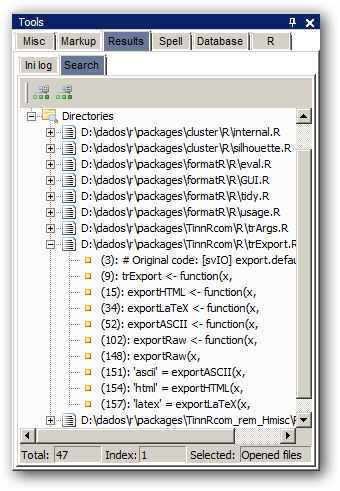
\includegraphics[scale=0.35]{./res/tools_results_search.png}
  \caption{Search (Tools/Results).}
  \label{fig:tools_results_search}
\end{figure}

The interface
(Figure \ref{fig:tools_results_search})
for \textit{Search} results associated with \textit{Search in files}.

The results for the \textit{Search in files} actions are displayed
as a tree with all files. Double click the file to open it in
the editor interface.


\hypertarget{working_tools_spell}{}
\subsection{Spell}
\index{tools interface!spell}

\begin{figure}[h!]
  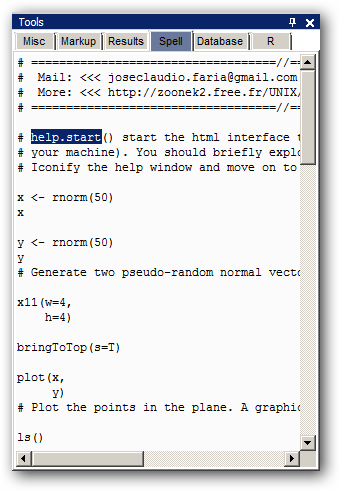
\includegraphics[scale=0.35]{./res/tools_spell.png}
  \caption{Spelling (Tools).}
  \label{fig:tools_spell}
\end{figure}

\begin{footnotesize}
  \begin{tabularx}{\textwidth}{>{\hsize=0.3\hsize}X>{\hsize=0.7\hsize}X}\\
    \hline
    \textbf{Tool} & \textbf{Description} \\
    \hline
    Spell & Interface to speller \\
    \hline
    \\
  \end{tabularx}
\end{footnotesize}

To enable spellchecking with Tinn-R it is necessary to install at
least one dictionary of the list of
\htmladdnormallink{available}{http://www.luziusschneider.com/Speller/English/index.htm} ones.
It is also a good idea to install the dictionary manager.
\htmladdnormallink{See instructions ...}{\#configuration\_spellerinstalation}.


\hypertarget{working_tools_database}{}
\subsection{Database}
\index{tools interface!database}

\begin{figure}[h!]
  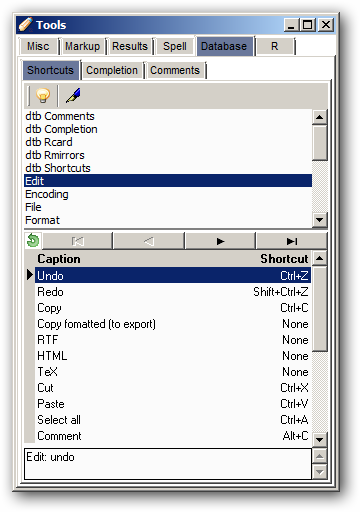
\includegraphics[scale=0.35]{./res/tools_database_shortcuts.png}~~
  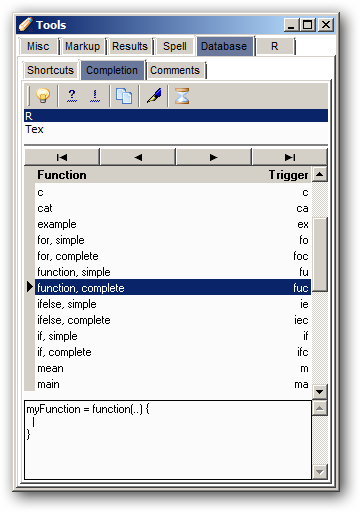
\includegraphics[scale=0.35]{./res/tools_database_completion.png}~~
  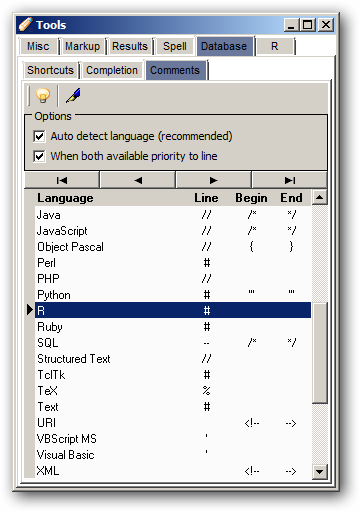
\includegraphics[scale=0.35]{./res/tools_database_comments.png}\\
  \caption{Database (Tools).}
  \label{fig:tools_database_options}
\end{figure}

\begin{table}
  \begin{footnotesize}
    \begin{tabularx}{\textwidth}{>{\hsize=0.3\hsize}X>{\hsize=0.7\hsize}X}\\
      \hline
      \textbf{Tool} & \textbf{Description} \\
      \hline
      Shortcuts & A digital shortcuts interface based in a XML database \\
      Completion & A digital completion interface based in a XML database \\
      Comments & A digital comments interface based in a XML database \\
      \hline
      \\
    \end{tabularx}
  \end{footnotesize}
  \caption{Database (Tools)}
  \label{tab:tools_database_options}
\end{table}


The database
(Figure \ref{fig:tools_database_options} and
Table \ref{tab:tools_database_options})
uses the native XML engine provided by Borland. Each tab
(\textit{Shortcuts}, \textit{Completion} and
\textit{Comments}) has its own pop-up menus and toolbars.


\subsubsection{Shortcuts:}

The \textit{Shortcuts} interface allows the user to find out about
the internal organization of Tinn-R and also to customize all
shortcuts related to the application. It is our intention, in
the near future, to add additional keystrokes related to the
editor and to the \RR{} hotkeys.


\subsubsection{Completion:}

The \textit{Completion} resource is very simple and allows high level
of user customization related to edition. The old implementation of
completion resource showed instability and was replaced. We hope that
the users will like this new one.

\subsubsection{Comments:}

The \textit{Comments} resource is very simple and allows high level
of user customization.

From version 3.0.1.0 Tinn-R automatically recognizes the
language of the file on focus. Further, inside the file
- if it is a syntax a multi-highlighter (complex syntax) - which language of
the line where the cursor (or selection) is found.

This identification is done automatically if (and only if) the option
\textit{(x) Auto detect language (recomended)} is checked. Otherwise
the user is forcing the application to use the comments of the selected language
(indicator arrow).

Selected code snippets involving more than one language will not be commented/uncommented
and a warning message is issued. That is, you must select only the snippet of a single language.


\hypertarget{working_tools_r}{}
\subsection{R}
\index{R!explorer}

\begin{figure}[h!]
  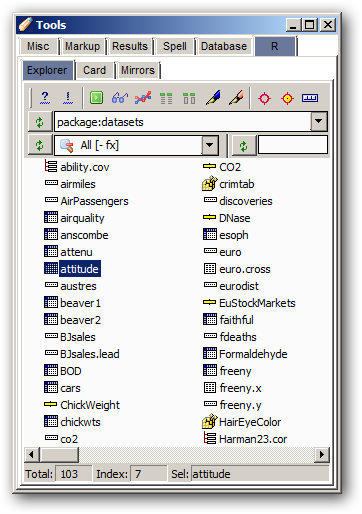
\includegraphics[scale=0.35]{./res/tools_r_explorer.png}~~
  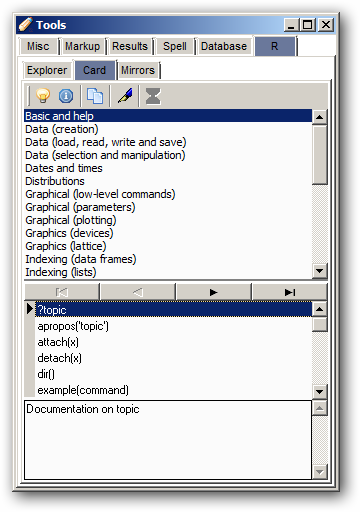
\includegraphics[scale=0.35]{./res/tools_r_card.png}~~
  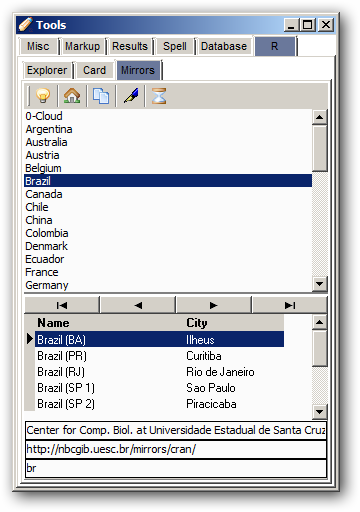
\includegraphics[scale=0.35]{./res/tools_r_mirrors.png}\\
  \caption{R (Tools).}
  \label{fig:tools_r}
\end{figure}

\begin{table}
  \begin{footnotesize}
    \begin{tabularx}{\textwidth}{>{\hsize=0.3\hsize}X>{\hsize=0.7\hsize}X}\\
      \hline
      \textbf{Tool} & \textbf{Description} \\
      \hline
      Explorer & Simple and functional graphical interface of objects of the \RR{} environment \\
      Card & A digital and simple \RR{} card based in a XML database \\
      Mirrors & A digital and simple \RR{} mirrors management based in a XML database \\
      \hline
      \\
    \end{tabularx}
  \end{footnotesize}
  \caption{R (Tools).}
  \label{tab:tools_r}
\end{table}

A simple and functional graphical interface
(Figure \ref{fig:tools_r} and
Table \ref{tab:tools_r})
of objects, card and mirrors management of the \RR{} environment.


\newpage
\subsubsection{Explorer:}
\index{R!explorer}

This interface
(Figure \ref{fig:tools_r})
has its own pop-up menu, toolbar and three combo box. The
pop-up menu and toolbar contain the most common actions related to an object
explorer.

The button \textit{R explorer: refresh environment} sends an instruction to
\RR{} environment requesting the list of all loaded packages in the current
session. The result is shown inside a graphical classified list. When one
of these is selected, the graphical list (and structure) of the objects
are shown.

There are two options of filter: type of objects and any sequence of
characters associated with the names of the objects.

It is possible to remove visible objects of the user workspace (.GlobalEnv)
using the key \textit{Delete}. To do this, select an object and type
\textit{Delete}.

A double click in any selected object will add its name to the editor.
If the object is dragged to the editor interface, the textual description
of the object is always shown in a new file. It is useful to know the
sources of functions and to see data objects (vectors, frames, list, etc).

\subsubsection{Card:}
\index{R!card}

The \textit{card} was based on two \RR{} cards already published:
R/Rpad Reference Card by Tom Short and \RR{} reference card by Jonathan Baron.

\begin{figure}[h!]
  \includegraphics[scale=0.35]{./res/rcard_dlg.png}\\
  \caption{R card (Database).}
  \label{fig:rcard_dlg}
\end{figure}

The available buttons
(Figure \ref{fig:tools_r})
are:

\begin{quote}
  \begin{footnotesize}
    \begin{description}
      \item[Help:]
        Sends the following instruction to \RR{}: \texttt{help('selected function')}.
      \item[Example:]
        Sends the following instruction to \RR{}: \texttt{example('selected function')}.
      \item[Copy function:]
        Places the selected function in the clipboard.
      \item[Copy descrition:]
        Places the descrition of the selected function on the clipboard.
      \item[Edit:]
        Opens the dialog \textit{R card database (xml based)} below.
      \item[Insert:]
        Inserts the selected function in the active editor. A
        \texttt{Double click} or \texttt{Enter} performs the same function.
    \end{description}
  \end{footnotesize}
\end{quote}

The \textit{Edit} button opens the dialog shown in the Figure \ref{fig:rcard_dlg}.

Read below a brief description of available buttons:

\begin{quote}
  \begin{footnotesize}
    \begin{description}
      \item[Restore default:]
        Restores the file \texttt{Rcard.xml} from the origin at
        (\texttt{InstallPath/data/data.zip}). Any prior changes in the
        file \texttt{Rcard.xml} currently being used will be lost.
      \item[New:]
        Places the table in insertion mode.
      \item[Delete:]
        Delete the current registry from the table.
      \item[Edit:]
        Places the table in edition mode.
      \item[Cancel current:]
        Cancels any change made to the current edition.
      \item[Cancel all:]
        Cancels all changes made to the database prior to \textit{Save}.
      \item[Save:]
        Overwrites the text file (XML) saving all changes made to the current table.
      \item[Close:]
        Closes the dialog. All non-saved changes will be lost.
    \end{description}
  \end{footnotesize}
\end{quote}


\subsubsection{Mirrors:}
\index{R!mirror}

The \textit{Mirrors} is an interface that allows the user to manage the repositories (or mirrors) of \RR{}.
You should always choose a repository physically closest to where you are,
so that, the Web communication tends to be faster and more efficient.

The default mirror is the University \htmladdnormallink{Wien}{http://cran.at.r-project.org/}
(Austria). Consider that this is the central mirror of CRAN.

The reasons for the Tinn-R always set a repository are two:
\begin {itemize}
   \item Prevent \RR{} keep asking which repository you want to use in each session;
   \item Workaround of intermittency (only Rterm) display the dialog for selecting the repository.
    That is, sometimes the dialog is displayed and not others. The cause of this intermittency is still unknown.
\end {itemize}

\begin{figure}[h!]
  \includegraphics[scale=0.35]{./res/mirrors_dlg.png}\\
  \caption{R mirrors (Database).}
  \label{fig:mirrors_dlg}
\end{figure}

The available buttons
(Figure \ref{fig:tools_r})
are:

\begin{quote}
  \begin{footnotesize}
    \begin{description}
      \item[Help:]
        Opens the User guide.
      \item[Update:]
        Updates the available \RR{} mirrors.
      \item[Copy host:]
        Places the selected mirror host in the clipboard.
      \item[Copy URL:]
        Places the selected mirror URL in the clipboard.
      \item[Edit:]
        Opens the dialog \textit{R mirrors (xml based)} below.
      \item[Insert:]
        Sends the following instruction to \RR{}: \texttt{options('repos='URL of selected mirror')}.
    \end{description}
  \end{footnotesize}
\end{quote}

The \textit{Edit} button opens the dialog shown in the Figure \ref{fig:mirrors_dlg}.

Read below a brief description of available buttons:

\begin{quote}
  \begin{footnotesize}
    \begin{description}
      \item[Restore default:]
        Restores the file \texttt{Rmirrors.xml} from the origin at
        (\texttt{InstallPath/data/data.zip}). Any prior change to the
        file \texttt{Rmirrors.xml} while being used will be lost.
      \item[New:]
        Places the table in insertion mode.
      \item[Delete:]
        Deletes the current registry from the table.
      \item[Edit:]
        Places the table in edition mode.
      \item[Cancel current:]
        Cancels any change made during the current editing session.
      \item[Cancel all:]
        Cancels all changes made to the database prior to \textit{Save}.
      \item[Save:]
        Overwrites the text file (XML) while saving all changes made to the current table.
      \item[Close:]
        Closes the dialog. All changes not previously saved will be lost.
    \end{description}
  \end{footnotesize}
\end{quote}

\newpage

\hypertarget{working_filetabs}{}
\section{File tabs}
\index{filetabs}

\begin{figure}[h!]
  \includegraphics[scale=0.35]{./res/filetabs.png}\\
  \caption{File tabs.}
  \label{fig:filetabs}
\end{figure}

\begin{figure}[h!]
  \includegraphics[scale=0.35]{./res/filetabs_menu.png}\\
  \caption{File tabs menu.}
  \label{fig:filetabs_menu}
\end{figure}

The position of the file tabs
(Figure \ref{fig:filetabs})
can be changed by drag and drop. It allows to
put the file tab in a desirable order making it suitable for the user interface.

The file tabs have itheir own pop-up menu
(Figure \ref{fig:filetabs_menu})
allowing fast control of the most common tasks.

\newpage

\hypertarget{working_toolsbar}{}
\section{Tools bar}
\index{toolsbar}

\begin{figure}[h!]
  \includegraphics[scale=0.35]{./res/toolsbar.png}\\
  \caption{Tools bar.}
  \label{fig:toolsbar}
\end{figure}

\begin{table}[h!]
  \begin{footnotesize}
    \begin{tabularx}{\textwidth}{>{\hsize=0.3\hsize}X>{\hsize=0.7\hsize}X}\\
      \hline
      \textbf{Category} & \textbf{Description} \\
      \hline
      File & New, open, save, save all, reload and print \\
      Edit & Undo and redo \\
      Filter & Create a new file with all occurrences of typed sequence of characters \\
      Macro & Record and play \\
      Misc & On top, focus control and block marks \\
      Processing & Conversion, compilation and viewer \\
      \RR{} & Lots of options to send and control \RR{} \\
      Search & Current file, in files, replace and go to line \\
      Syntax & Drop down list of all syntaxes available \\
      Spell & Drop down list of installed dictionaries and a bottom to start the speller \\
      View & Organize screen, Tools (show/hide), Tools (size), Rterm (show/hide, Rterm (size), options to \textit{IO} and \textit{Log} and word wrap \\
      \hline
    \end{tabularx}
  \end{footnotesize}
  \caption{Tools bar.}
  \label{tab:toolsbar}
\end{table}

Unlike most applications of this category, this interface
(Figure \ref{fig:toolsbar})
was designed to be
as small and simple as possible. In other words, the full access to all
resources of Tinn-R are available at the main menu and associated shortcuts
(it takes time to learn all and most are user configurable).

Two groups are available: main and \RR{} tool bar.

The main toolbar interface is categorized
(Table \ref{tab:toolsbar})
and contains the most common tasks:

The \RR{} toolbar has two basic divisions: Send (left side, finishing in the
\textit{Set work directory buttom}) and Control (right side, starting
in the \textit{List all objects buttom}).


\hypertarget{working_toolsbar_showhide}{}
\subsection{Show/Hide}
\index{toolsbar!showhide}

\begin{figure}[h!]
  \includegraphics[scale=0.35]{./res/toolsbar_pmenu.png}\\
  \caption{Tools bar menu.}
  \label{fig:toolsbar_pmenu}
\end{figure}

The Tools bar has its own pop-up
(Figure \ref{fig:toolsbar_pmenu})
menu enabling the user to choose what
resources will be visible (show/hide). To see the pop-up menu, press the
right mouse buttom inside any place of the main tool bar.


\hypertarget{working_toolsbar_disposition}{}
\subsection{Disposition}
\index{toolsbar!disposition}

The interface also allows drag and drop. In other words, you can organize
the order of the individual tool bar inside of the main container.

It is better to do that with the main interface not maximized to avoid
screen flicker (a small nuance related to some version of the Windows
and Borland engine).

\newpage

\hypertarget{working_findreplace}{}
\section{Find and replace}
\index{find and replace}

\begin{figure}[h!]
  \includegraphics[scale=0.35]{./res/find.png}~~
  \includegraphics[scale=0.35]{./res/replace.png}\\
  \caption{Find and replace dialog.}
  \label{fig:find_replace}
\end{figure}

The dialogs for \textit{Find}
and \textit{Replace}
(Figure \ref{fig:find_replace})
are very similar, so this session will just discuss the \textit{Replace} dialog
and will point out the changes when necessary.


\subsection{Find}
When you call up the \textit{Find} dialog
the \textit{Find for} box will be
prefilled with the word under the cursor. You can type over the entry if you
are looking for another word. There is also a dropdown list of phrases
previously searched.


\subsection{Replace (Replace dialog only)}
When you call up the \textit{Replace} dialog
the \textit{Replace with} box
will be filled with the last string you entered in it. If this is the first
time you have called the \textit{Replace} dialog since starting Tinn-R then
the Replace box will be empty. You can type over any text in box. There is
also a dropdown list of strings previously used.


\subsubsection{Options:}

\begin{quote}
  \begin{footnotesize}
    \begin{description}
      \item[Case sensitive:]
        When this option is set the search is done case sensitively. For instance,
        \texttt{Ab}, \texttt{AB} and \texttt{ab} are all treated as different words
        whereas they are not if the option is not set.
      \item[Whole words only:]
        When this option is set the system will only find complete words matching
        the search criteria. So, for example, if \texttt{ab} is the search string
        the system will not match occurrences of words like \texttt{abc} or
        \texttt{cab}.
      \item[Regular expressions:]
        \htmladdnormallink{See regular expressions ...}{\#working\_regularexpressions}
    \end{description}
  \end{footnotesize}
\end{quote}


\subsubsection{Direction:}

The direction to search. This option is ignored if searching in selected text.

\begin{quote}
  \begin{footnotesize}
    \begin{description}
      \item[Forward:]
        Search from the cursor position to the end of the file.
      \item[Backward:]
        Search from the cursor position to the beginning of the file.
    \end{description}
  \end{footnotesize}
\end{quote}


\subsubsection{Scope:}
\begin{quote}
  \begin{footnotesize}
    \begin{description}
      \item[Global:]
        Search the entire file.
      \item[Selected Text:]
        Search just the selected text.
    \end{description}
  \end{footnotesize}
\end{quote}


\subsubsection{Origin:}
\begin{quote}
  \begin{footnotesize}
    \begin{description}
      \item[Global:]
        Search from the beginning of the file.
      \item[From cursor:]
        Search just from the position of the cursor.
    \end{description}
  \end{footnotesize}
\end{quote}

\newpage

\hypertarget{working_searchinfiles}{}
\section{Search in files}
\index{search!in files}

\begin{figure}[h!]
  \includegraphics[scale=0.35]{./res/searchinfiles.png}~~
  \includegraphics[scale=0.35]{./res/tools_results_search.png}\\
  \caption{Search in files.}
  \label{fig:searchinfiles}
\end{figure}


The \textit{Search in files} dialog
(Figure \ref{fig:searchinfiles})
allows you to match a criteria in all opened files and/or in files on disk.


\subsection{Options}
\index{search!case sensitivity}
\index{search!regular expressions}

\begin{quote}
  \begin{footnotesize}
    \begin{description}
      \item[Case sensitive:]
        When this option is set the search is case sensitive.
        For example, \texttt{Ab}, \texttt{AB} and \texttt{ab}
        are all treated as different words.
      \item[Whole words only:]
        When this option is set the system will only find complete
        words matching the search criteria. For example, if
        \texttt{ab} is the search string the system will not match
        occurrences of words such as \texttt{abc} or \texttt{cab}.
      \item[Regular expressions:]
        \htmladdnormallink{See regular expressions ...}{\#working\_regularexpressions}
    \end{description}
  \end{footnotesize}
\end{quote}


\subsection{Where}

\begin{quote}
  \begin{footnotesize}
    \begin{description}
      \item[Opened files:]
        When this option is set the search is performed on all opened files.
      \item[Directories:]
        When this option is set the search is performed in disk files.
    \end{description}
  \end{footnotesize}
\end{quote}


\subsection{Directory options}

\begin{quote}
  \begin{footnotesize}
    \begin{description}
      \item[Directory:]
        A dropdown list of previously searched directories.
      \item[File mask:]
        A dropdown list of the previously searched file mask.
      \item[Search in sub directories:]
        When this option is set the search is performed on all sub
        directories of the main directory.
    \end{description}
  \end{footnotesize}
\end{quote}


\subsection{Results interface}
\index{search!results}

The associated results interface
(Figure \ref{fig:searchinfiles})
shows the results.

A double click in a single occurrence (or dragging and dropping it into the
editor interface) will open the file and results will be placed in the first
line of the editor window.

\newpage

\hypertarget{working_databases}{}
\section{Databases}
\index{databases}

All databases uses the native XML engine provided by Borland.

\subsection{Shortcuts}
\index{databases!shortcuts}

\begin{figure}[h!]
  \includegraphics[scale=0.35]{./res/shortcuts_dlg.png}\\
  \caption{Shortcuts (Databases).}
  \label{fig:shortcuts_dlg_2}
\end{figure}

Read below for a brief description of available buttons (Figure \ref{fig:shortcuts_dlg_2}):

\begin{quote}
  \begin{footnotesize}
    \begin{description}
      \item[Restore default:]
        Restores the file \texttt{Shortcuts.xml} from the origin
        (InstallPath/data/data.zip). Any prior changes to the file
        \texttt{Shortcuts.xml} currently being used will be lost.
      \item[Save as default:]
        Opens the save dialog allowing you to save the file. From
        this point on, this file will be the new default shortcut.
      \item[Load:]
        Opens the open dialog allowing you to load a shortcut file.
        From this point on, this file will be the new default shortcut.
      \item[Edit:]
        Places the table in edition mode.
      \item[Cancel current:]
        Cancels any change made to the current edition.
      \item[Cancel all:]
        Cancels all changes made to the database prior to \textit{Save} or \textit{Save as default}.
      \item[Save:]
        Overwrites the text file (XML) saving all changes made to the current table.
      \item[Close:]
        Closes the dialog. All non-saved changes will be lost.
    \end{description}
  \end{footnotesize}
\end{quote}


\subsection{Completion}
\index{databases!completion}

\begin{figure}[h!]
  \includegraphics[scale=0.35]{./res/completion_dlg.png}\\
  \caption{Completion (Databases).}
  \label{fig:completion_dlg}
\end{figure}

This resource adds a granular level of user customization for editing
all within Tinn-R.

The completion (database based) allows the user to add functions based
on several programming languages such as \RR{}, \TeX, among others.

Read below for a brief description of available buttons (Figure \ref{fig:completion_dlg}):

\begin{quote}
  \begin{footnotesize}
    \begin{description}
      \item[Restore default:]
        Restores the file \texttt{Completion.xml} from the origin at
        (\texttt{InstallPath/data/data.zip}). Any prior change to the file
        \texttt{Completion.xml} being used will be lost.
      \item[New:]
        Places the table in insertion mode.
      \item[Delete:]
        Deletes the current registry from the table.
      \item[Edit:]
        Places the table in edition mode.
      \item[Cancel current:]
        Cancels any change made to the current edition.
      \item[Cancel all:]
        Cancels all changes made to the database prior to \textit{Save}.
      \item[Save:]
        Overwrites the text file (XML), saving all changes made to the current table.
      \item[Close:]
        Closes the dialog. All non-saved changes will be lost.
    \end{description}
  \end{footnotesize}
\end{quote}


\subsection{Comments}
\index{databases!comments}

\begin{figure}[h!]
  \includegraphics[scale=0.35]{./res/comments_dlg.png}\\
  \caption{Comments (Databases).}
  \label{fig:comments_dlg}
\end{figure}

The \textit{Comments} resource is very simple and allows high level
of user customization.

From version 3.0.1.0 Tinn-R automatically recognizes the
language of the file on focus. Further, inside the file
- if it is a syntax a multi-highlighter (complex syntax) - which language of
the line where the cursor (or selection) is found.

This identification is done automatically if (and only if) the option
\textit{(x) Auto detect language (recomended)} is checked. Otherwise
the user is forcing the application to use the comments of the selected language
(indicator arrow).

Selected code snippets involving more than one language will not be commented/uncommented
and a warning message is issued. That is, you must select only the snippet of a single language.

Read below a brief description of available buttons (Figure \ref{fig:comments_dlg}):

\begin{quote}
  \begin{footnotesize}
    \begin{description}
      \item[Restore default:]
        Restores the file \texttt{Comments.xml} from the origin at
        (\texttt{InstallPath/data/data.zip}). Any prior changes in the
        file \texttt{Comments.xml} currently being used will be lost.
      \item[Edit:]
        Places the table in edition mode.
      \item[Cancel current:]
        Cancels any change made to the current edition.
      \item[Cancel all:]
        Cancels all changes made to the database prior to \textit{Save}.
      \item[Save:]
        Overwrites the text file (XML) saving all changes made to the current table.
      \item[Close:]
        Closes the dialog. All non-saved changes will be lost.
    \end{description}
  \end{footnotesize}
\end{quote}


\subsection{Card (R)}
\index{R!card}
\index{databases!card (R)}

The \textit{card} was based on two \RR{} cards already published:
R/Rpad Reference Card by Tom Short and \RR{} reference card by Jonathan Baron.

\begin{figure}[h!]
  \includegraphics[scale=0.35]{./res/rcard_dlg.png}\\
  \caption{R card (Databases).}
  \label{fig:rcard_dlg_1}
\end{figure}

Read below a brief description of available buttons (Figure \ref{fig:rcard_dlg_1}):

\begin{quote}
  \begin{footnotesize}
    \begin{description}
      \item[Restore default:]
        Restores the file \texttt{Rcard.xml} from the origin at
        (\texttt{InstallPath/data/data.zip}). Any prior changes in the
        file \texttt{Rcard.xml} currently being used will be lost.
      \item[New:]
        Places the table in insertion mode.
      \item[Delete:]
        Delete the current registry from the table.
      \item[Edit:]
        Places the table in edition mode.
      \item[Cancel current:]
        Cancels any change made to the current edition.
      \item[Cancel all:]
        Cancels all changes made to the database prior to \textit{Save}.
      \item[Save:]
        Overwrites the text file (XML) saving all changes made to the current table.
      \item[Close:]
        Closes the dialog. All non-saved changes will be lost.
    \end{description}
  \end{footnotesize}
\end{quote}


\subsection{Mirrors (R)}
\index{R!mirror}
\index{databases!mirrors (R)}

The \textit{Mirrors} is an interface that allows the user to manage the repositories (or mirrors) of \RR{}.
You should always choose a repository physically closest to where you are,
so that, the Web communication tends to be faster and more efficient.

The default mirror is the University \htmladdnormallink{Wien}{http://cran.at.r-project.org/}
(Austria). Consider that this is the central mirror of CRAN.

The reasons for the Tinn-R always set a repository are two:
\begin {itemize}
   \item Prevent \RR{} keep asking which repository you want to use in each session;
   \item Workaround of intermittency (only Rterm) display the dialog for selecting the repository.
    That is, sometimes the dialog is displayed and not others. The cause of this intermittency is still unknown.
\end {itemize}

\begin{figure}[h!]
  \includegraphics[scale=0.35]{./res/mirrors_dlg.png}\\
  \caption{R mirrors (Databases).}
  \label{fig:mirrors_dlg_1}
\end{figure}

Read below a brief description of available buttons (Figure \ref{fig:mirrors_dlg_1}):

\begin{quote}
  \begin{footnotesize}
    \begin{description}
      \item[Restore default:]
        Restores the file \texttt{Rmirrors.xml} from the origin at
        (\texttt{InstallPath/data/data.zip}). Any prior change to the
        file \texttt{Rmirrors.xml} while being used will be lost.
      \item[New:]
        Places the table in insertion mode.
      \item[Delete:]
        Deletes the current registry from the table.
      \item[Edit:]
        Places the table in edition mode.
      \item[Cancel current:]
        Cancels any change made during the current editing session.
      \item[Cancel all:]
        Cancels all changes made to the database prior to \textit{Save}.
      \item[Save:]
        Overwrites the text file (XML) while saving all changes made to the current table.
      \item[Close:]
        Closes the dialog. All changes not previously saved will be lost.
    \end{description}
  \end{footnotesize}
\end{quote}

\newpage

\hypertarget{working_regularexpressions}{}
\section{Regular expressions}
\index{regular expressions}

This session is an adaptation. It is based on the help of the
freewere \htmladdnormallink{PSPad}{http://www.pspad.com/} editor.


\subsection{What are regular expressions?}

\textit{Regular expressions} are widely-used method to specify text patterns
to be searched for. Special metacharacters allow you to specify, for
instance, that a particular string you are looking for occurs at the
beginning or end of a line, or contains n recurrences of a certain character.

Regular expressions may look ugly to novices, but are actually a very simple,
handy and powerful tool.


\subsection{Simple Matches}
\index{regular expressions!simple matches}

Any single character matches itself, unless it is a metacharacter with a
special meaning described below.

A series of characters matches that series of characters in the target
string, so the pattern \texttt{bluh} would match \texttt{bluh} in the
target string.

You can cause characters that normally function as metacharacters or
escape sequences to be interpreted literally by \texttt{escaping} them.
Do this by preceding them with a backslash \texttt{$\backslash$}. For
instance: metacharacter \texttt{\^{}} match beginning of string, but
\texttt{$\backslash$\^{}} match character \texttt{\^{}},
\texttt{$\backslash$$\backslash$} match \texttt{$\backslash$} and so on.


\subsubsection{Examples:}

\begin{footnotesize}
  \begin{tabularx}{\textwidth}{>{\hsize=0.3\hsize}X>{\hsize=0.7\hsize}X}\\
    \hline
    \textbf{ER} & \textbf{Matches} \\
    \hline
    \texttt{foobar} & \texttt{foobar} \\
    \texttt{$\backslash$\^{}FooBarPtr} & \texttt{\^{}FooBarPtr} \\
    \hline
  \end{tabularx}
\end{footnotesize}


\subsection{Escape Sequences}
\index{regular expressions!escape sequences}

Characters may be specified using a escape sequences syntax much like that
used in C and Perl: \texttt{$\backslash$n} matches a newline,
\texttt{$\backslash$t} a tab, etc. More generally, \texttt{$\backslash$xnn},
where \texttt{nn} is a string of hexadecimal digits, matches the character
whose ASCII value is \texttt{nn}. If you need wide (Unicode) character code,
you can use \texttt{$\backslash$x\{nnnn\}}, where \texttt{nnnn} is one or
more hexadecimal (base 16) digits (1, 2, 3, 4, 5, 6, 7, 8, 9, A, B, C, D, E, F).
Hex digit letters may be in upper or lower case.

\begin{footnotesize}
  \begin{tabularx}{\textwidth}{>{\hsize=0.3\hsize}X>{\hsize=0.7\hsize}X}\\
    \hline
    \textbf{ER} & \textbf{Description} \\
    \hline
    \texttt{$\backslash$xnn} & Char with hex code \texttt{nn} \\
    \texttt{$\backslash$x\{nnnn\}} & Char with hex code \texttt{nnnn} (one byte for plain text and two bytes for Unicode) \\
    \texttt{$\backslash$t} & Tab (HT/TAB), same as \texttt{$\backslash$x09} \\
    \texttt{$\backslash$n} & Newline (NL), same as \texttt{$\backslash$x0a} \\
    \texttt{$\backslash$r} & Carriage return (CR), same as \texttt{$\backslash$x0d} \\
    \texttt{$\backslash$f} & Form feed (FF), same as \texttt{$\backslash$x0c} \\
    \texttt{$\backslash$a} & Alarm (bell) (BEL), same as \texttt{$\backslash$x07} \\
    \texttt{$\backslash$e} & Escape (ESC), same as \texttt{$\backslash$x1b} \\
    \hline
    \\
  \end{tabularx}
\end{footnotesize}


\subsubsection{Examples:}

\begin{footnotesize}
  \begin{tabularx}{\textwidth}{>{\hsize=0.3\hsize}X>{\hsize=0.7\hsize}X}\\
    \hline
    \textbf{ER} & \textbf{Matches} \\
    \hline
    \texttt{foo$\backslash$x20bar} & \texttt{foo bar} (note space in the middle) \\
    \texttt{$\backslash$tfoobar} & \texttt{foobar} predefined by tab \\
    \hline
    \\
  \end{tabularx}
\end{footnotesize}


\subsection{Character Classes}
\index{regular expressions!character classes}

You can specify a character class by enclosing a list of characters in
\texttt{[]}, which will match any one character from the list. If the
first character after the \texttt{[} is \texttt{\^{}}, the class matches
any character not in the list.


\subsubsection{Examples:}

\begin{footnotesize}
  \begin{tabularx}{\textwidth}{>{\hsize=0.3\hsize}X>{\hsize=0.7\hsize}X}\\
    \hline
    \textbf{ER} & \textbf{Matches} \\
    \hline
    \texttt{foob[aeiou]r} & \texttt{foobar}, \texttt{foober}, etc. But not \texttt{foobbr}, \texttt{foobcr}, etc \\
    \texttt{foob[\^{}aeiou]r} & \texttt{foobbr}, \texttt{foobcr}, etc. But not \texttt{foobar}, \texttt{foober}, etc \\
    \hline
    \\
  \end{tabularx}
\end{footnotesize}

Within a list, the \texttt{-} character is used to specify a range, so
that \texttt{a-z} represents all characters between \texttt{a} and
\texttt{z}, inclusive.

If you want \texttt{-} itself to be a member of a class, put it at the
start or end of the list, or escape it with a backslash. If you want
\texttt{]} you may place it at the start of list or escape it with a
backslash.


\subsubsection{Examples:}

\begin{footnotesize}
  \begin{tabularx}{\textwidth}{>{\hsize=0.3\hsize}X>{\hsize=0.7\hsize}X}\\
    \hline
    \textbf{ER} & \textbf{Matches} \\
    \hline
    \texttt{[-az]} & \texttt{a}, \texttt{z} and \texttt{-} \\
    \texttt{[az-]} & \texttt{a}, \texttt{z} and \texttt{-} \\
    \texttt{[a$\backslash$-z]} & \texttt{a}, \texttt{z} and \texttt{-} \\
    \texttt{[a-z]} & All twenty six small characters from \texttt{a} to \texttt{z} \\
    \texttt{[$\backslash$n-$\backslash$x0D]} & Any of ASCII \texttt{\#10(Lf)}, \texttt{\#11}, \texttt{\#12(Ff)}, \texttt{\#13(Cr)} \\
    \texttt{[$\backslash$d-t]} & Any digit, \texttt{-} or \texttt{t} \\
    \texttt{[]-a]} & Any char from \texttt{]}..\texttt{a} \\
    \hline
    \\
  \end{tabularx}
\end{footnotesize}


\subsection{Metacharacters}
\index{metacharacters}

Metacharacters are special characters which are the essence of regular
expressions. There are different types of metacharacters, described below.


\subsubsection{Metacharacters - Line Separators:}
\index{metacharacters!line separators}

\begin{footnotesize}
  \begin{tabularx}{\textwidth}{>{\hsize=0.3\hsize}X>{\hsize=0.7\hsize}X}\\
    \hline
    \textbf{ER} & \textbf{Description} \\
    \hline
    \texttt{\^{}} & Start of line \\
    \texttt{\$} & End of line \\
    \texttt{$\backslash$A} & Start of text \\
    \texttt{$\backslash$Z} & End of text \\
    \texttt{.} & Any character in line \\
    \hline
    \\
  \end{tabularx}
\end{footnotesize}


\subsubsection{Examples:}

\begin{footnotesize}
  \begin{tabularx}{\textwidth}{>{\hsize=0.3\hsize}X>{\hsize=0.7\hsize}X}\\
    \hline
    \textbf{ER} & \textbf{Matches} \\
    \hline
    \texttt{\^{}foobar} & \texttt{foobar} only if it's at the beginning of line \\
    \texttt{foobar\$} & \texttt{foobar} only if it's at the end of line \\
    \texttt{\^{}foobar\$} & \texttt{foobar} only if it's the only string in line \\
    \texttt{foob.r} & \texttt{foobar}, \texttt{foobbr}, \texttt{foob1r} and so on \\
    \hline
    \\
  \end{tabularx}
\end{footnotesize}

The \texttt{\^{}} metacharacter by default is only guaranteed to match at
the beginning of the input string/text, the \texttt{\$} metacharacter
only at the end. Embedded line separators will not be matched by
\texttt{\^{}} or \texttt{\$}. You may, however, wish to treat a string
as a multi-line buffer, such that the \texttt{\^{}} will match after
any line separator within the string, and \texttt{\$} will match before
any line separator. You can do this by switching the modifier \texttt{/m} on.

The \texttt{$\backslash$A} and \texttt{$\backslash$Z} are just like
\texttt{\^{}} and \texttt{\$}, except that they won't match multiple
times when the modifier \texttt{/m} is used, while \texttt{\^{}} and
\texttt{\$} will match at every internal line separator.


\subsubsection{Metacharacters - Predefined Classes:}
\index{metacharacters!predefined classes}

\begin{footnotesize}
  \begin{tabularx}{\textwidth}{>{\hsize=0.3\hsize}X>{\hsize=0.7\hsize}X}\\
    \hline
    \textbf{ER} & \textbf{Description} \\
    \hline
    \texttt{$\backslash$w} & An alphanumeric character (including \texttt{\_}) \\
    \hline
    \texttt{$\backslash$W} & A non alphanumeric character \\
    \texttt{$\backslash$d} & A numeric character \\
    \texttt{$\backslash$D} & A non-numeric character \\
    \texttt{$\backslash$s} & Any space (same as \texttt{[ $\backslash$t$\backslash$n$\backslash$r$\backslash$f])} \\
    \texttt{$\backslash$S} & A non space \\
    \hline
    \\
  \end{tabularx}
\end{footnotesize}

You may use $\backslash$w, $\backslash$d and $\backslash$s within
custom character classes.


\subsubsection{Examples:}

\begin{footnotesize}
  \begin{tabularx}{\textwidth}{>{\hsize=0.2\hsize}X>{\hsize=0.9\hsize}X}\\
    \hline
    \textbf{ER} & \textbf{Matches} \\
    \hline
    \texttt{foob$\backslash$dr} & \texttt{foob1r}, \texttt{foob6r} and so on but not \texttt{foobar}, \texttt{foobbr} and so on \\
    \texttt{foob[$\backslash$w$\backslash$s]r} & \texttt{foobar}, \texttt{foob r}, \texttt{foobbr} and so on but not \texttt{foob1r}, \texttt{foob=r} and so on \\
    \hline
    \\
  \end{tabularx}
\end{footnotesize}

TRegExpr uses properties SpaceChars and WordChars to define character
classes \texttt{$\backslash$w}, \texttt{$\backslash$W},
\texttt{$\backslash$s}, \texttt{$\backslash$S}, so you can easily
redefine it.


\subsubsection{Metacharacters - Word Boundaries:}
\index{metacharacters!word boundaries}

\begin{footnotesize}
  \begin{tabularx}{\textwidth}{>{\hsize=0.3\hsize}X>{\hsize=0.7\hsize}X}\\
    \hline
    \textbf{ER} & \textbf{Matches} \\
    \hline
    \texttt{$\backslash$b} & A word boundary \\
    \texttt{$\backslash$B} & A non-(word boundary) \\
    \hline
    \\
  \end{tabularx}
\end{footnotesize}

A word boundary \texttt{$\backslash$b} is a spot between two characters
that has a \texttt{$\backslash$w} on one side of it and a \texttt{$\backslash$W}
on the other side of it (in either order), counting the imaginary characters
of the beginning and end of the string as matching a \texttt{$\backslash$W}.


\subsubsection{Metacharacters - Iterators:}
\index{metacharacters!iterators}

Any item of a regular expression may be followed by another type of
metacharacters - iterators. Using this metacharacters you can specify
number of occurrences of the previous character, metacharacter or subexpression.

\begin{footnotesize}
  \begin{tabularx}{\textwidth}{>{\hsize=0.3\hsize}X>{\hsize=0.7\hsize}X}\\
    \hline
    \textbf{ER} & \textbf{Matches} \\
    \hline
    \texttt{*} & Zero or more ("greedy"), similar to \{0,\} \\
    \texttt{+} & One or more ("greedy"), similar to \{1,\} \\
    \texttt{?} & Zero or one ("greedy"), similar to \{0,1\} \\
    \texttt{\{n\}} & Exactly n times ("greedy") \\
    \texttt{\{n,\}} & At least n times ("greedy") \\
    \texttt{\{n,m\}} & At least n but not more than m times ("greedy") \\
    \texttt{*?} & At least n but not more than m times ("greedy") \\
    \texttt{+?} & At least n but not more than m times ("greedy") \\
    \texttt{??} & Zero or one ("non-greedy"), similar to \{0,1\}? \\
    \texttt{\{n\}?} & Exactly n times ("non-greedy") \\
    \texttt{\{n,\}?} & At least n times ("non-greedy") \\
    \texttt{\{n,m\}?} & At least n but not more than m times ("non-greedy") \\
    \hline
    \\
  \end{tabularx}
\end{footnotesize}

So, digits in curly brackets of the form \texttt{\{n,m\}}, specify the
minimum number of times to match the item n and the maximum m. The form
\texttt{\{n\}} is equivalent to \texttt{\{n,n\}} and matches exactly n
times. The form \texttt{\{n,\}} matches n or more times. There is no
limit to the size of n or m, but large numbers will chew up more memory
and slow down r.e. execution.

If a curly bracket occurs in any other context, it is treated as a
regular character.


\subsubsection{Examples:}

\begin{footnotesize}
  \begin{tabularx}{\textwidth}{>{\hsize=0.3\hsize}X>{\hsize=0.7\hsize}X}\\
    \hline
    \textbf{ER} & \textbf{Matches} \\
    \hline
    \texttt{foob.*r} & \texttt{foobar}, \texttt{foobalkjdflkj9r} and \texttt{foobr} \\
    \texttt{foob.+r} & \texttt{foobar}, \texttt{foobalkjdflkj9r} but not \texttt{foobr} \\
    \texttt{foob.?r} & \texttt{foobar}, \texttt{foobbr} and \texttt{foobr} but not \texttt{foobalkj9r} \\
    \texttt{fooba\{2\}r} & \texttt{foobaar} \\
    \texttt{fooba\{2,\}r} & \texttt{foobaar}, \texttt{foobaaar}, \texttt{foobaaaar}, ... \\
    \texttt{fooba\{2,3\}r} & \texttt{foobaar}, or \texttt{foobaaar} but not \texttt{foobaaaar} \\
    \hline
    \\
  \end{tabularx}
\end{footnotesize}

A little explanation about \texttt{greediness}. \texttt{Greedy} takes as
many as possible, \texttt{non-greedy} takes as few as possible. For
example, \texttt{b+} and \texttt{b*} applied to string \texttt{abbbbc}
return \texttt{bbbb}, \texttt{b+?} returns \texttt{b}, \texttt{b*?}
returns empty string, \texttt{b\{2,3\}?} returns \texttt{bb},
\texttt{b\{2,3\}} returns \texttt{bbb}.


\subsubsection{Metacharacters - Alternatives:}
\index{metacharacters!alternatives}

You can specify a series of alternatives for a pattern using \texttt{$|$}
to separate them, so that fee$|$fie$|$foe will match any of \texttt{fee},
\texttt{fie}, or \texttt{foe} in the target string (as would f(e$|$i$|$o)e).
The first alternative includes everything from the last pattern delimiter
(\texttt{(}, \texttt{[}, or the beginning of the pattern) up to the first
\texttt{$|$}, and the last alternative contains everything from the last
\texttt{$|$} to the next pattern delimiter. For this reason, it's common
practice to include alternatives in parentheses, to minimize confusion
about where they start and end.

Alternatives are tried from left to right, so the first alternative found
for which the entire expression matches, is the one that is chosen. This
means that alternatives are not necessarily greedy. For example: when
matching foo$|$foot against \texttt{barefoot}, only the \texttt{foo} part
will match, as that is the first alternative tried, and it successfully
matches the target string. (This might not seem important, but it is
important when you are capturing matched text using parentheses).

Also remember that \texttt{$|$} is interpreted as a literal within square
brackets, so if you write \texttt{[fee$|$fie$|$foe]}. You're really only
matching \texttt{[feio$|$]}.


\subsubsection{Examples:}

\begin{footnotesize}
  \begin{tabularx}{\textwidth}{>{\hsize=0.3\hsize}X>{\hsize=0.7\hsize}X}\\
    \hline
    \textbf{ER} & \textbf{Matches} \\
    \hline
    \texttt{foo(bar$|$foo)} & \texttt{foobar} or \texttt{foofoo} \\
    \hline
    \\
  \end{tabularx}
\end{footnotesize}


\subsubsection{Metacharacters - Subexpressions:}
\index{metacharacters!subexpressions}

The bracketing construct ( ... ) may also be used to define r.e.
subexpressions (after parsing, you can find subexpression positions,
lengths and actual values in MatchPos, MatchLen and Match properties
of TRegExpr, and substitute it in clip strings by TRegExpr.Substitute).

Subexpressions are numbered based on the left to right order of their
opening parenthesis. First subexpression has number \texttt{1} (whole
r.e. match has number \texttt{0} - you can substitute it in TRegExpr.
Substitute as \texttt{\$0} or \texttt{\$\&}).


\subsubsection{Examples:}

\begin{footnotesize}
  \begin{tabularx}{\textwidth}{>{\hsize=0.3\hsize}X>{\hsize=0.7\hsize}X}\\
    \hline
    \textbf{ER} & \textbf{Matches} \\
    \hline
    \texttt{(foobar)\{8,10\}} & Strings which contain 8, 9 or 10 instances of the \texttt{foobar} \\
    \texttt{foob([0-9]$|$a+)r} & \texttt{foob0r}, \texttt{foob1r} , \texttt{foobar}, \texttt{foobaar}, \texttt{foobaar}, ... \\
    \texttt{(abc(def)ghi(123))xzy} & \texttt{abcdefghi123xyz} (the only match) \\
    \hline
    \\
  \end{tabularx}
\end{footnotesize}


\subsubsection{Then backreferences:}
\index{metacharacters!backreferences}

\begin{footnotesize}
  \begin{tabularx}{\textwidth}{>{\hsize=0.3\hsize}X>{\hsize=0.7\hsize}X}\\
    \hline
    \textbf{ER} & \textbf{Description} \\
    \hline
    \texttt{$\backslash$1} & \texttt{= abcdefghi123} \\
    \texttt{$\backslash$2} & \texttt{=def} \\
    \texttt{$\backslash$3} & \texttt{=123} \\
    \texttt{$\backslash$0} & \texttt{=abcdefghi123xyz (the whole match)} \\
    \hline
  \end{tabularx}
\end{footnotesize}

We could find the same string using metacharacter Iterators with:
(\texttt{$\backslash$w\{3\}([d-f]\{3\})...($\backslash$d*))xyz} and the
backreferences would have the same values. And yet the pattern would
also match: \texttt{123fdd@\#\$4444xyz}, \texttt{bbbeeeabc1234567xyz},
\texttt{ddddddaaaxyz}.


\subsubsection{Metacharacters - Backreferences:}
\index{metacharacters!backreferences}

Metacharacters \texttt{$\backslash$1} through \texttt{$\backslash$9}
are interpreted as backreferences in the \textit{Search text} box. When
used outside of the regular expression, such as in the \textit{Replace
  text} field, metacharacters \texttt{\$1} through \texttt{\$9} are
interpreted as backreferences to the last find.

\texttt{$\backslash$$<$n$>$} matches previously matched subexpression
\texttt{\#$<$n$>$}.


\subsubsection{Find Examples:}
\index{metacharacters!find examples}

\begin{footnotesize}
  \begin{tabularx}{\textwidth}{>{\hsize=0.3\hsize}X>{\hsize=0.7\hsize}X}\\
    \hline
    \textbf{ER} & \textbf{Matches} \\
    \hline
    \texttt{(.)$\backslash$1+} & \texttt{aaaa} and \texttt{cc} \\
    \texttt{(.+)$\backslash$1+} & \texttt{abab} and \texttt{123123} \\
    \texttt{(['"]?)($\backslash$d+)$\backslash$1} & \texttt{"13"}(in double quotes),
    or \texttt{'4'} (in single quotes) or \texttt{77} (without quotes), ... \\
    \hline
  \end{tabularx}
\end{footnotesize}

\begin{quote}
  \begin{footnotesize}
    \begin{description}
      \item[Replace Examples:]
        Date format change from \texttt{dd.mm.yyyy} to \texttt{yyyy-mm-dd}. This will
        turn the European date style \texttt{26.8.1994} or \texttt{26/8/1994}
        into \texttt{1994-8-26}.
        Search: \texttt{([0-9]\{1,2\}).([0-9]\{1,2\}).([0-9]\{4\})}
        Replace: \texttt{\$3-\$2-\$1}
        Make sure you check the box for \textit{Regular Expression}.
    \end{description}
  \end{footnotesize}
\end{quote}


\subsection{Regular Expression Tutorials}

The following is a list of a few sites that contain tutorials on both regular
expressions in general and their use in specific languages:

\begin{itemize}
  \item \htmladdnormallink{General Tutorial}{http://www.regular-expressions.info/}
  \item \htmladdnormallink{Regular Expressions - User guide}{http://www.zytrax.com/tech/web/regex.htm}
  \item \htmladdnormallink{Regular Expression HOWTO}{http://docs.python.org/2/howto/regex.html}
  \item \htmladdnormallink{Perl Regular Expressions}{http://www.troubleshooters.com/codecorn/littperl/perlreg.htm}
  \item \htmladdnormallink{Regular Expression Basic Syntax Reference}{http://www.regular-expressions.info/reference.html}
\end{itemize}

